%!TEX TS-program = pdflatex
\PassOptionsToPackage{a4paper,margin=1in}{geometry}
\documentclass[sn-vancouver,Numbered]{sn-jnl}

\usepackage{amsmath,amssymb}
\usepackage{booktabs}
\usepackage{graphicx}
\usepackage{multirow}
\usepackage{tabularx}
\usepackage{threeparttable}
\usepackage{url}
\usepackage{xcolor}

\hypersetup{
  pdftitle={Adaptive Governance, Oracle Latency, and Automated Risk Engine Design for Local-Currency DeFi Lending Protocols},
  pdfauthor={Niko Rokni Lamouki; Salma Soofiyan},
  pdfsubject={Adaptive governance and oracle stress testing for hypothetical local-currency DeFi lending},
  pdfkeywords={decentralized finance, local-currency stablecoins, adaptive governance, price oracles, circuit breakers, protocol risk}
}

\newcommand{\lcu}{\mathrm{LCU}}
\newcommand{\usd}{\mathrm{USD}}
\newcommand{\clip}{\operatorname{clip}}
\newcommand{\E}{\mathbb{E}}

\begin{document}

\title[Adaptive Governance and Oracle Architecture]{Adaptive Governance, Oracle Latency, and Automated Risk Engine Design for Local-Currency DeFi Lending Protocols}

\author*[1]{\fnm{Niko} \sur{Rokni Lamouki}}
\email{nrokni@uel.ac.uk}
\author[1]{\fnm{Salma} \sur{Soofiyan}}

\affil*[1]{\orgdiv{School of Architecture, Computing and Engineering},
\orgname{University of East London},
\orgaddress{\street{Docklands Campus}, \city{London}, \postcode{E16 2RD},
\country{United Kingdom}}}

\abstract{Local-currency decentralized-finance (DeFi) lending creates a control problem that does not arise in the same form for a deep, continuously traded USD stablecoin. The protocol must distinguish an official foreign-exchange reference from the price at which users can actually sell the token, combine feeds that update at different speeds, and change risk parameters before debt issuance amplifies a market dislocation. We design and stress-test an automated risk engine that maps estimated collateral volatility, decentralized-exchange (DEX) basis, oracle disagreement, and utilisation into bounded updates of the borrowing rate, debt ceiling, and liquidation ratio. A three-source median oracle and a circuit breaker are evaluated against a static single-oracle benchmark, a 48-hour delayed decentralized-autonomous-organization (DAO) benchmark, and an adaptive design without a breaker. Calibration uses 42 joint monthly Argentine-peso (ARS), Turkish-lira (TRY), and ETH returns from January 2020 to July 2023. Monthly observations are preserved exactly while adverse moves are assigned to random six-hour intervals. The main experiment contains 6,000 four-month moving-block bootstrap paths per currency and architecture, supplemented by 39 realised rolling windows, attack, latency, official--parallel-rate, governance-delay, and controller-ablation exercises. In the stated counterfactual, static single-oracle bad-debt probability is 15.4\% for ARS and 14.0\% for TRY; the full architecture reduces it to 0.28\% and 0.20\%. A DEX discount above 10\% occurs in every static and 48-hour delayed-DAO path. The full architecture reduces this severe-depeg probability to zero for ARS and 25.0\% for TRY. Protection is costly: new borrowing is paused in 28.0\% and 29.1\% of six-hour intervals, and cumulative credit falls from approximately 0.70 to 0.20--0.22 initial-ceiling units. A one-source attack twice the baseline magnitude raises pooled static bad-debt probability from 14.4\% to 20.4\%, while the robust architecture remains at 0.33\%. The residual TRY failures show that governance cannot manufacture arbitrage balance sheet or settlement capacity: an automated controller can stop endogenous issuance, but it cannot guarantee a peg when background conversion flow alone overwhelms the market. The estimates are reproducible design stresses, not forecasts or evidence from a deployed ARS- or TRY-denominated protocol.}

\keywords{Decentralized finance, local-currency stablecoins, adaptive governance, price oracles, circuit breakers, foreign exchange, protocol risk, moving-block bootstrap}

\maketitle

\section{Introduction}\label{sec:introduction}

In DeFi lending, a parameter is part of the solvency mechanism. A borrowing rate changes the incentive to create debt; a debt ceiling limits the protocol's exposure to an asset and its surrounding market; a liquidation ratio determines how much price movement can occur before collateral is sold. These parameters are often encoded in smart contracts, yet their levels or functional forms remain subject to governance. A token-holder vote, risk-committee recommendation, governance spell, and security delay can be appropriate for structural changes. The same sequence can be too slow when collateral falls, an exchange-rate reference becomes stale, or an on-chain venue is manipulated within hours.

The timing problem is sharper for a hypothetical stablecoin denominated in a high-inflation local currency. At least three prices coexist. The \emph{official reference} determines the declared local-currency value; the \emph{parallel or executable reference} reflects the price at which hard currency may actually be obtained; and the \emph{DEX price} reflects the balance sheets, liquidity, and settlement access of on-chain intermediaries. These prices can separate exactly when users have the greatest incentive to draw a local-currency liability and exchange it for USDC or another hard-currency asset. A delayed official feed may be manipulation-resistant but economically unrepresentative. A thin DEX feed may be current but manipulable. Medianization reduces one-source attacks, but a median of stale or institutionally different prices is not automatically a ground truth.

This paper is the fourth in a sequence on local-currency DeFi lending. The first paper estimated the counterfactual erosion of ARS- and TRY-denominated debt using public MakerDAO ETH-A borrowing events \cite{RokniLamouki2026Debt}. The second added joint FX and crypto-collateral shocks, interest accrual, liquidation, bad debt, and reserves \cite{RokniLamouki2026Solvency}. The third separated the official reference from a DEX execution price and studied liquidity-provider participation, finite arbitrage capital, and redemption capacity \cite{RokniLamouki2026Peg}. Those papers exposed a remaining assumption: they applied policy parameters mechanically and did not make the governance/oracle loop itself an object of design.

Real protocols illustrate the institutional relevance. Aave defines borrow caps, collateral factors, and liquidation thresholds as risk parameters monitored by service providers and adjustable by governance \cite{AaveReserve,AaveRisk}. Maker/Sky executive actions have changed debt ceilings, fees, and liquidation parameters and can be subject to a governance security-module delay; an October 2024 executive notice, for example, reported a 16-hour delay \cite{MakerVote2024}. Chainlink data feeds update under deviation and heartbeat rules rather than as continuous streams and advise applications to verify timestamps and adopt a pause or alternate mode when answers are not sufficiently fresh \cite{ChainlinkFeeds}. Each mechanism is reasonable in isolation. Their joint behaviour under a moving FX reference, collateral jump, DEX discount, and governance delay is not obvious.

We ask four research questions:

\begin{description}
  \item[RQ1] How do oracle latency, one-source manipulation, and disagreement between official and executable FX prices affect valuation error, liquidation quality, and bad debt?
  \item[RQ2] Can a bounded automated controller for the borrowing rate, debt ceiling, and liquidation ratio reduce loss without creating unstable parameter oscillation?
  \item[RQ3] What incremental protection does a circuit breaker provide, and how much credit access does that protection consume?
  \item[RQ4] How rapidly does the benefit of adaptive governance deteriorate when parameter execution is delayed from six hours to conventional DAO time scales?
\end{description}

The contribution is a reproducible architecture comparison rather than a claim that one numerical rule is universally optimal. First, the model composes an official FX source, a DEX price, and an independent reference feed and makes cross-source disagreement a state variable. Second, it couples oracle quality to a lending book, opportunistic borrowing during manipulation, liquidation at contemporaneous true value, and a persistent DEX discount created by token sales. Third, it specifies a transparent risk score and rate-limited control law instead of a black-box policy. Fourth, it implements a breaker that pauses new draws while preserving repayments and collateral top-ups. Fifth, it separates loss reduction from the real option value of credit by reporting bad debt, severe depeg, accepted borrowing, rates, ceilings, and pause time together.

The main result is conditional but sharp. The full architecture materially reduces bad debt in both currencies, and it prevents a severe ARS depeg in the main simulation. It does not eliminate severe TRY depegs because some bootstrapped TRY moves generate background conversion pressure above arbitrage capacity before protocol-originated issuance can be stopped. This is a useful boundary: oracle engineering and governance speed can control endogenous exposure, but neither creates market depth. A safety claim that ignores this boundary would be stronger than the model supports.

\section{Related Literature and Research Gap}\label{sec:literature}

\subsection{Oracles, manipulation, and latency}

Smart contracts cannot observe off-chain prices without an oracle trust model. Eskandari et al. \cite{Eskandari2021} systematise the path from ground truth to on-chain use and show that data sourcing, aggregation, and update design each create attack surfaces. Flash-loan research demonstrates how temporarily moving a price can alter borrowing and liquidation within a single transaction or short interval \cite{Qin2021}. More recent oracle work seeks manipulation resistance with medians, time weighting, and multiple observation windows, but those defences create an accuracy--latency trade-off \cite{Bai2025}. Sadeghi and Feinstein \cite{Sadeghi2026} explicitly note that hardened mechanisms such as TWAPs and medianized feeds can delay liquidations during sharp declines.

Operational documentation reaches a similar conclusion from a different direction. Chainlink feeds expose an update timestamp because a correct historical answer can still be unsafe for an application that requires a current answer \cite{ChainlinkFeeds}. A robust integration therefore needs both \emph{value validation} and \emph{freshness validation}. Our architecture adds a third check: economic disagreement between price domains. This is important for a local-currency instrument because an official price and a parallel price can both be genuine observations of different settlement regimes.

\subsection{Algorithmic lending parameters and governance}

Protocols for loanable funds set rates and collateral conditions by code, while governance selects parameters and sometimes the rule itself \cite{Gudgeon2020,Werner2022}. Evidence from Compound shows that utilisation enters piecewise-linear interest-rate functions and that more volatile assets tend to receive steeper rules \cite{Chaudhary2023}. Chiu et al. \cite{Chiu2023} show theoretically that rigidity can amplify a price--liquidity feedback and that flexible smart-contract updates can restore a unique equilibrium in their setting.

Adaptive DeFi research provides more direct comparators. Auto.gov uses a reinforcement-learning agent to adjust lending parameters and reports improved simulated profitability during oracle attacks \cite{Xu2025}. Bastankhah et al. \cite{Bastankhah2024} separate a fast interest controller from a slower collateral planner and establish convergence and robustness properties. These approaches show that automation can be more responsive than manual votes. They also raise governance questions: which state variables are admissible, what happens under distribution shift, how are actions bounded, and who may stop the controller? We therefore use an interpretable monotone score, explicit parameter domains, and per-step rate limits. The objective is auditability of the comparative mechanism, not machine-learning performance.

\subsection{Stablecoin parity and local-currency execution}

Stablecoin parity depends on redemption access, liquidity, and arbitrage rather than the declared peg alone \cite{Lyons2023,Ma2023}. Emerging-market stablecoins add exchange controls, segmented settlement, and time-varying hard-currency demand \cite{Auer2023}. Aldasoro, Beltran, and Grinberg \cite{Aldasoro2026} show that stablecoin-implied FX prices can deviate from conventional FX prices and that intermediary capital conditions amplify the response to flows. These findings motivate a state variable for the official--parallel gap and a separate endogenous DEX basis.

The companion peg-stability analysis makes finite arbitrage and redemption capacity explicit \cite{RokniLamouki2026Peg}. The present paper holds market-depth assumptions transparent and asks what governance can still do: reduce issuance, increase its price, demand more collateral, or temporarily stop new draws. The residual depeg under the strongest controller is therefore not a coding failure. It is the model's test of whether exogenous conversion flow has crossed the market-capacity boundary.

\subsection{Research gap}

Existing work explains oracle attacks, adaptive interest rules, or stablecoin parity separately. The missing link is a path-dependent local-currency lending model in which (i) price sources represent different settlement domains; (ii) source latency and manipulation affect borrowing and liquidation; (iii) issuance feeds back into a DEX discount; (iv) three risk parameters move together; and (v) governance delay and circuit-breaker cost are measured on the same paths. Figure~\ref{fig:architecture} summarises the proposed system.

\begin{figure*}[t]
\centering
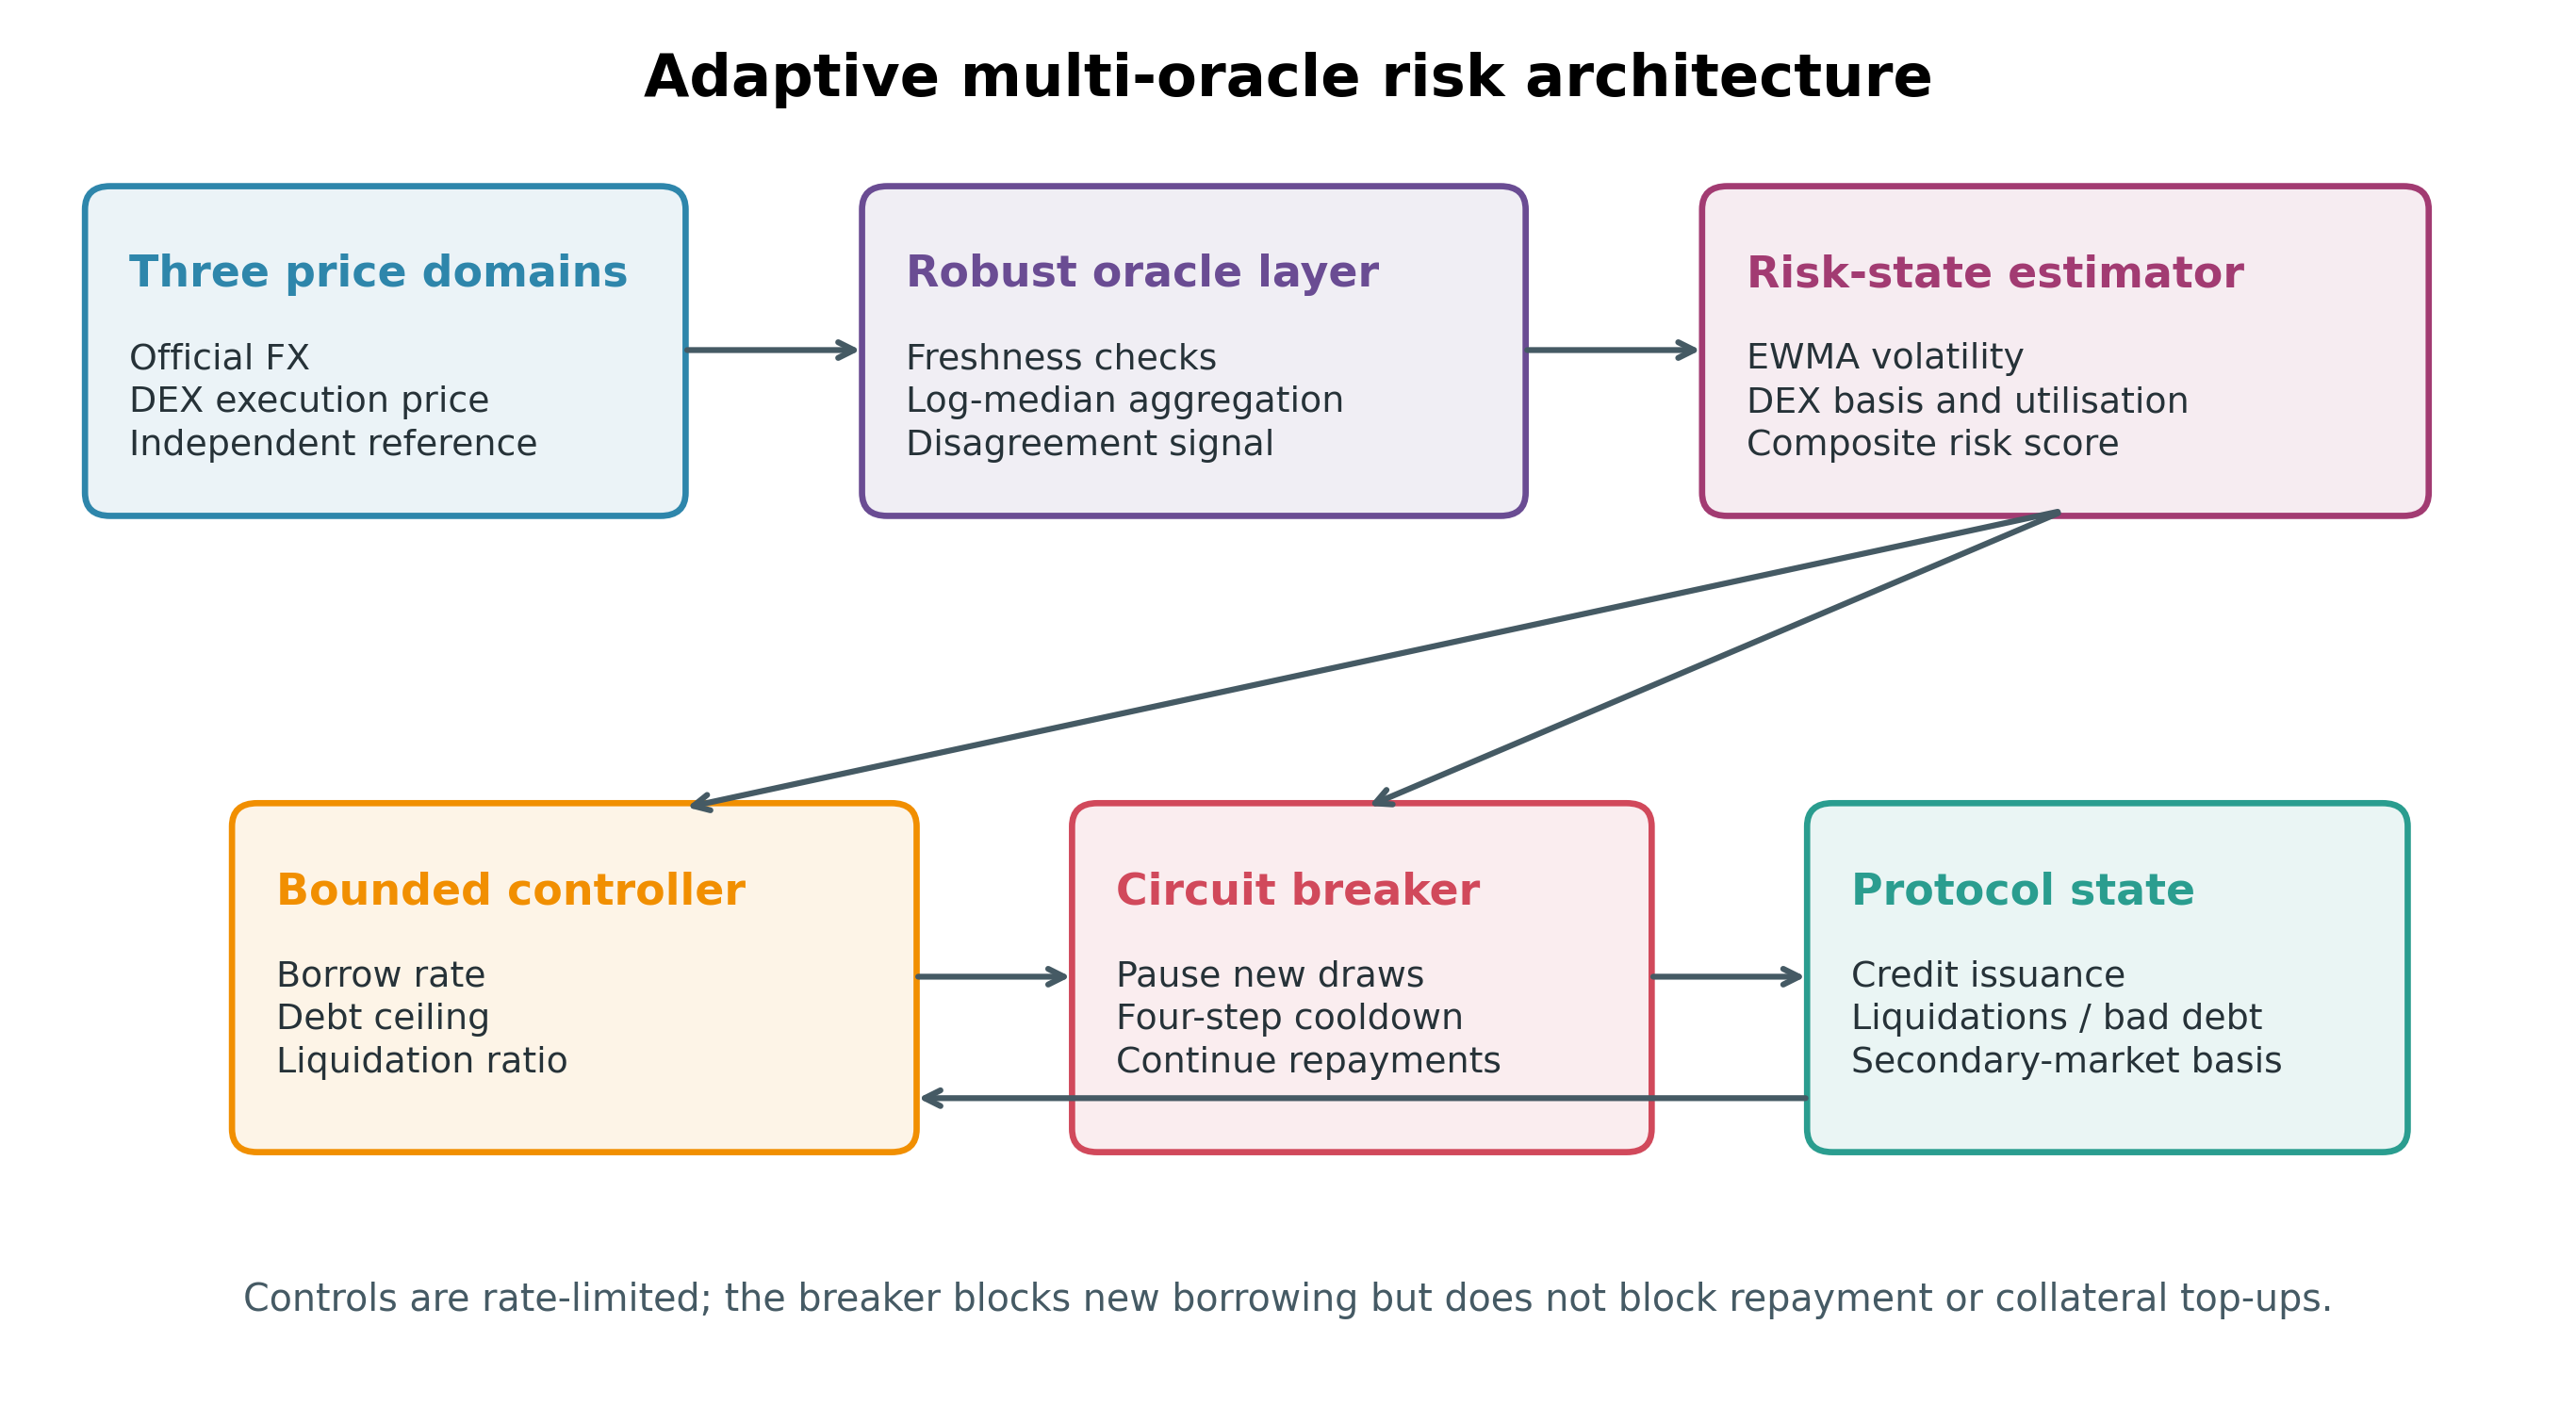
\includegraphics[width=\textwidth]{../figures/figure1_adaptive_architecture.png}
\caption{Adaptive multi-oracle risk architecture. The controller and breaker consume a common, auditable risk state. Protocol outcomes feed back into utilisation and the DEX basis.}
\label{fig:architecture}
\end{figure*}

\section{Institutional Design and Safety Objectives}\label{sec:design}

\subsection{Four architectures}

The experiment compares the architectures in Table~\ref{tab:architectures}. The \emph{static single-oracle} benchmark uses delayed official FX and a DEX collateral quote, fixed at an 8\% borrowing rate, unit debt ceiling, and 150\% liquidation ratio. It is intentionally fragile: the two legs have different governance and manipulation properties. The \emph{delayed DAO} uses a three-source median and computes the adaptive targets, but actions take effect after 48 hours. The \emph{adaptive multi-oracle} applies bounded actions every six hours. The \emph{adaptive multi + breaker} adds a 24-hour minimum cooldown for new draws after a trigger.

\begin{table*}[t]
\centering
\caption{Architecture comparison.}\label{tab:architectures}
\small
\begin{tabular}{p{3.2cm}p{4.0cm}p{3.2cm}p{2.6cm}}
\toprule
Architecture & Price aggregation & Parameter action & Breaker \\
\midrule
Static single & Official FX + DEX collateral & Fixed & No \\
Delayed DAO & Three-source median & 48-hour delay & No \\
Adaptive multi & Three-source median & Six-hour controller & No \\
Adaptive + breaker & Three-source median & Six-hour controller & Four-step cooldown \\
\bottomrule
\end{tabular}

\end{table*}

The breaker is deliberately asymmetric. It sets new borrowing to zero but continues to accept repayment and collateral top-ups. A symmetric pause could protect the protocol's accounting while preventing users from reducing risk; we exclude that unsafe design. Liquidation remains available because a collateral collapse can otherwise accumulate bad debt during the pause.

\subsection{Safety objectives and trade-offs}

The architecture has four objectives:

\begin{enumerate}
  \item minimise cumulative bad debt and the probability of a material loss event;
  \item keep the DEX discount below a severe-depeg threshold;
  \item avoid liquidation caused only by a mismatched or stale oracle; and
  \item preserve useful credit access, measured by accepted borrowing, ceiling, and unpaused time.
\end{enumerate}

No scalar objective is imposed ex ante because its weights would conceal distributional choices. Raising the liquidation ratio protects lenders but can liquidate borrowers. Lowering the ceiling protects the protocol but reduces credit. Raising the interest rate changes the timing and composition of demand. Pausing provides a hard bound on endogenous flow but removes the option to borrow during stress. Results therefore report a vector of outcomes rather than an optimised welfare score.

\section{Data and Reproducible Path Construction}\label{sec:data}

\subsection{Common calibration panel}

To preserve comparability with the companion papers, the analysis uses the same 43 monthly levels from January 2020 through July 2023 and 42 complete returns. ARS and TRY per USD are OECD Main Economic Indicators monthly exchange rates distributed by FRED \cite{FREDARS,FREDTRY}. ETH/USD is the Coin Metrics community series preserved in the companion solvency data package \cite{CoinMetrics}. Figure~\ref{fig:data} plots the levels and depreciation distributions, and Table~\ref{tab:data} reports summary statistics.

\begin{figure*}[t]
\centering
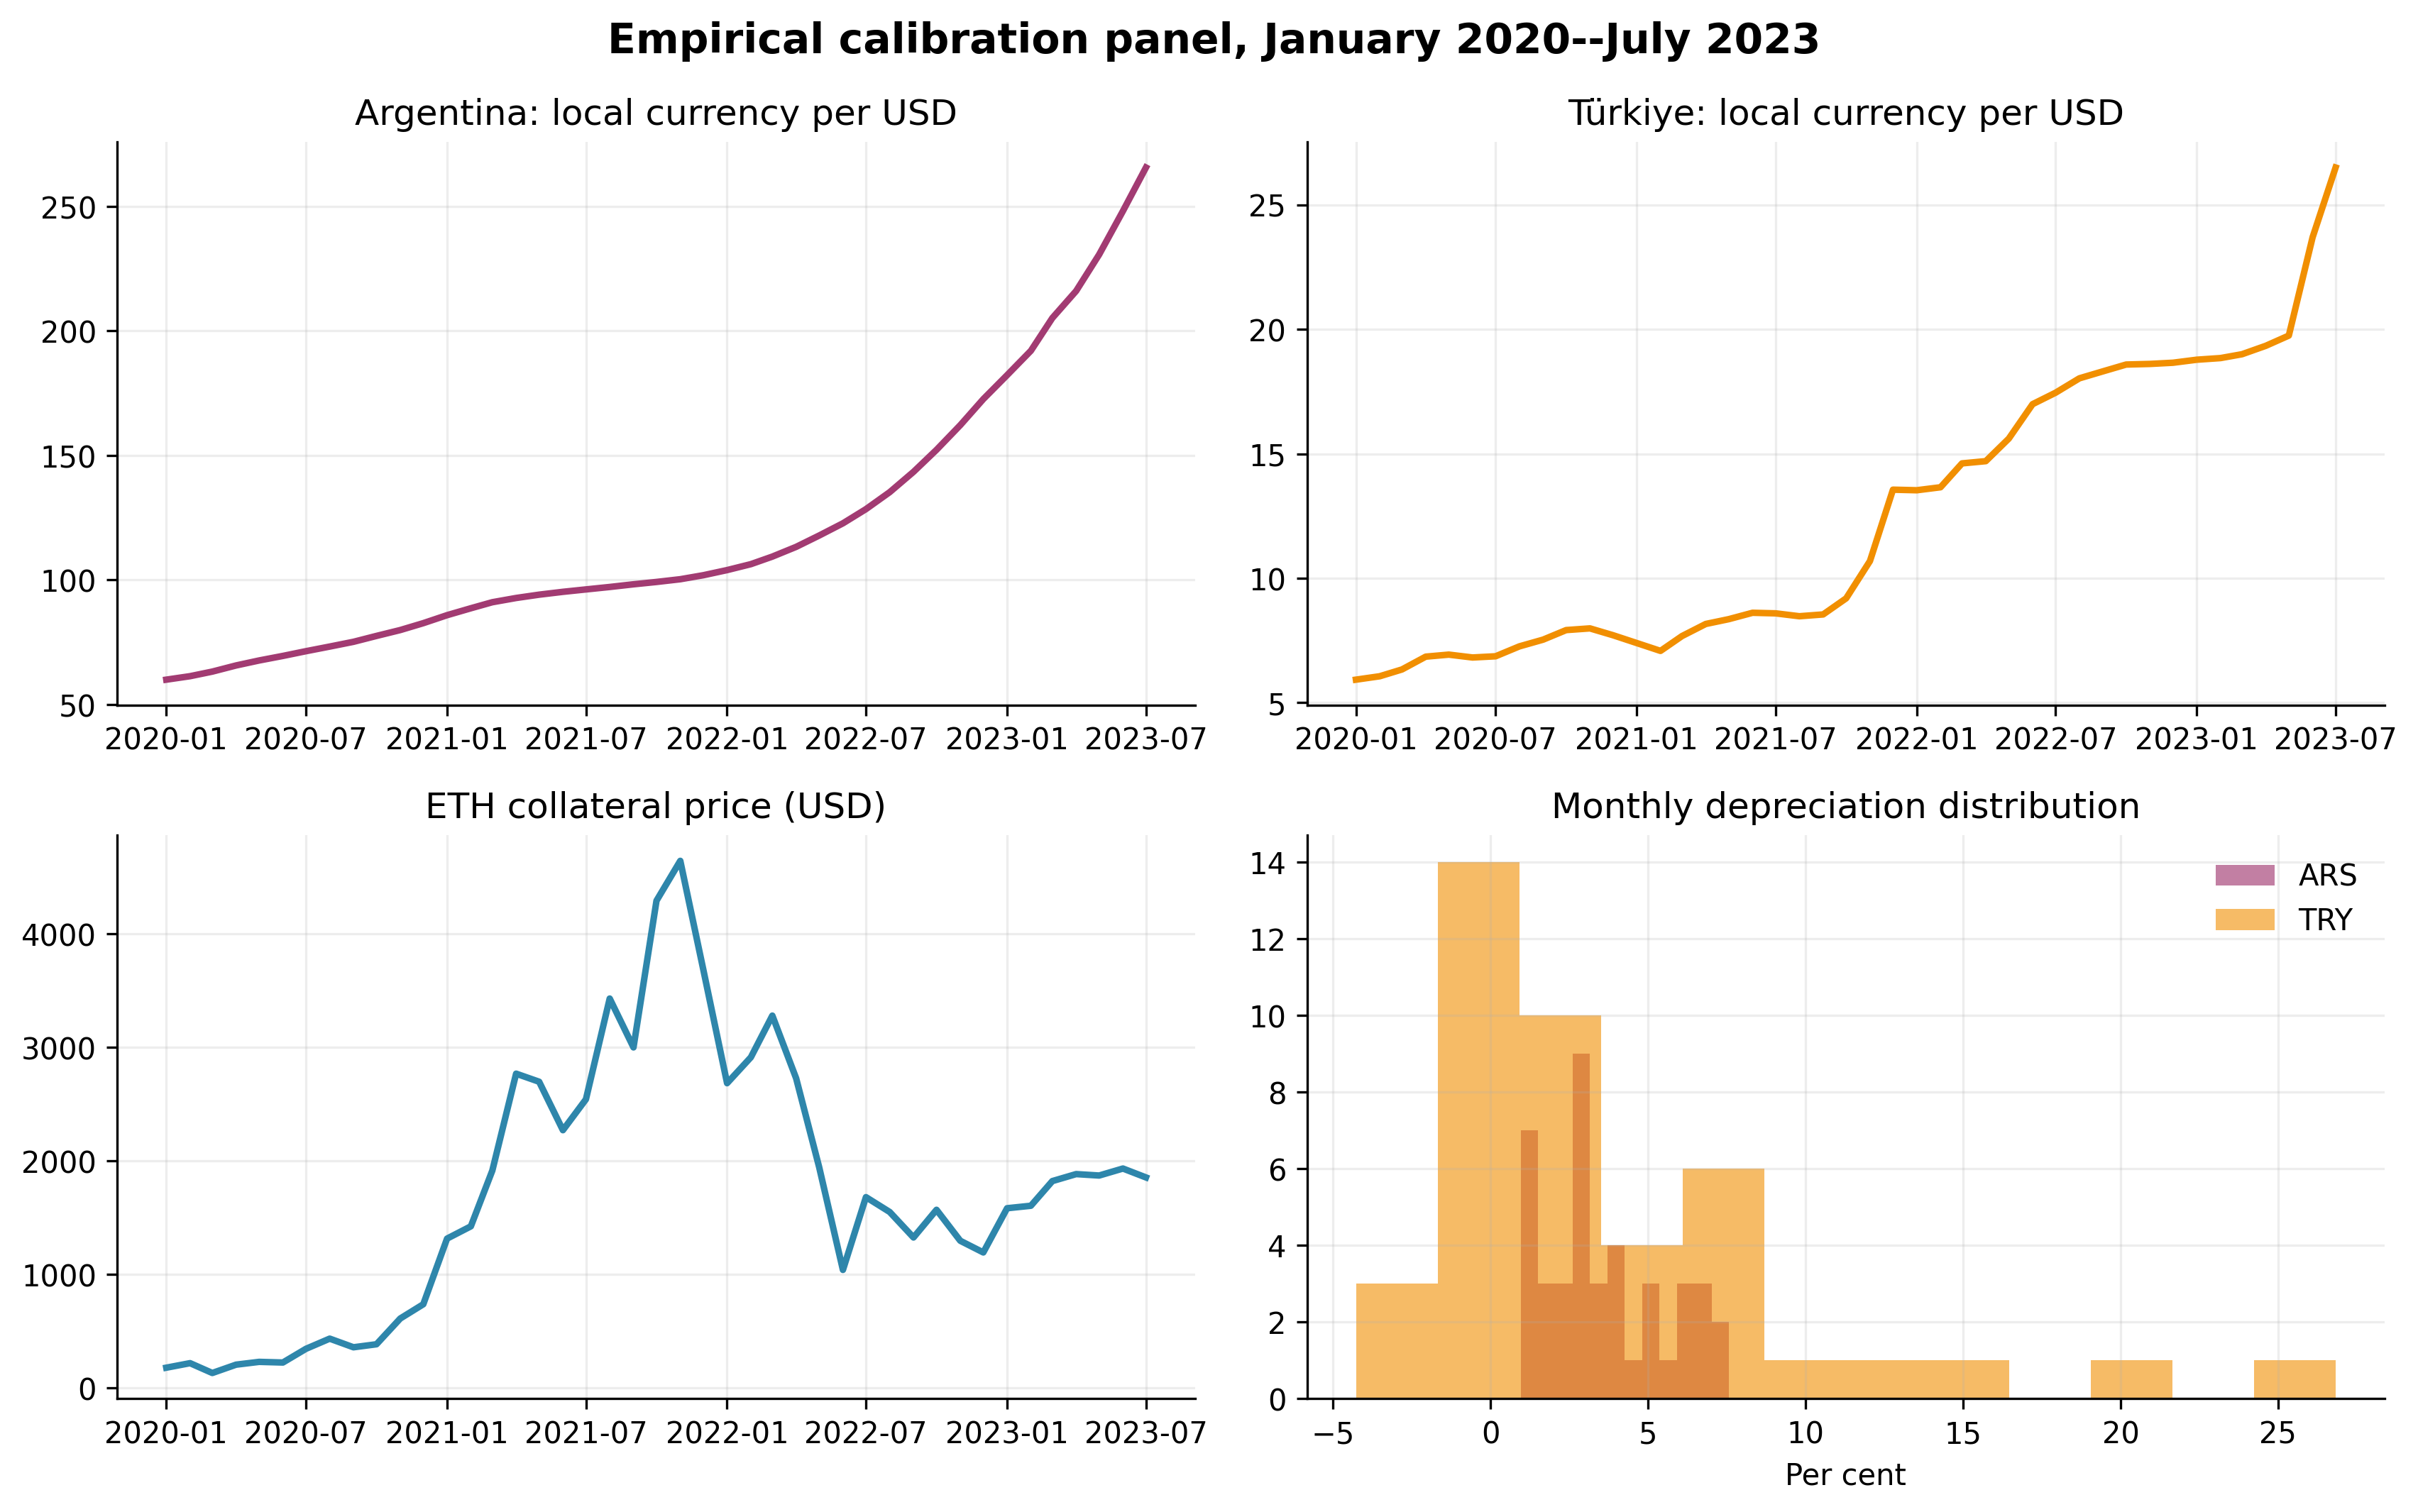
\includegraphics[width=\textwidth]{../figures/figure2_empirical_calibration.png}
\caption{Empirical calibration panel. Exchange-rate levels are reported as local-currency units per USD; a positive monthly change is local-currency depreciation.}
\label{fig:data}
\end{figure*}

\begin{table*}[t]
\centering
\caption{Monthly return summary, 42 observations.}\label{tab:data}
\small
\begin{tabular}{lrrrrr}
\toprule
Series & Observations & Mean & SD & Minimum & Maximum \\
\midrule
ARS depreciation & 42 & 3.62\% & 1.94\% & 0.96\% & 7.57\% \\
TRY depreciation & 42 & 3.79\% & 6.09\% & -4.27\% & 26.83\% \\
ETH return & 42 & 9.32\% & 28.40\% & -46.51\% & 78.25\% \\
\bottomrule
\end{tabular}

\end{table*}

The sample is intentionally inherited rather than extended opportunistically. This makes the fourth paper a controlled mechanism comparison on the same macro histories. It also limits external validity: results reflect a period containing the pandemic shock, crypto boom and drawdown, and substantial ARS and TRY depreciation, but not every capital-control or market-structure regime.

\subsection{Joint block sampling}

For currency $j\in\{\mathrm{ARS},\mathrm{TRY}\}$, let $z_m^j=(d_m^j,r_m^{\mathrm{ETH}})$ contain monthly local-currency depreciation and the matched ETH return. We sample circular two-month blocks of the joint vector using the moving-block bootstrap \cite{Kunsch1989}. The main horizon is four months. The same sampled path and intramonth random numbers are used for every architecture, making comparisons paired rather than independent.

All 39 overlapping realised four-month windows are also replayed. These windows are not independent observations and are not used for conventional standard errors. They are an audit layer showing how the mechanisms behave when the ordering of observed returns is retained.

\subsection{Six-hour bridge and jumps}

Oracle delay cannot be studied directly with monthly steps. Each sampled monthly log return is therefore disaggregated into 120 six-hour intervals. A centred Gaussian bridge supplies intramonth variation. When the monthly FX move is adverse, 60\% of its log decline is assigned to a random interval; the same rule applies to a negative ETH monthly return. A final mean correction guarantees

\begin{equation}
 \sum_{t\in m}\Delta\log p_t^{\lcu}=-\log(1+d_m),
 \qquad
 \sum_{t\in m}\Delta\log p_t^{C}=\log(1+r_m^{\mathrm{ETH}}),
 \label{eq:bridge}
\end{equation}

to machine precision. The bridge changes arrival time but not the bootstrapped monthly endpoint. This is a scenario generator, not observed high-frequency data. The distinction is enforced in the manuscript, source documentation, and validation tests.

\section{Oracle, Lending, and Control Model}\label{sec:model}

\subsection{True prices and price domains}

Let $p_t^{\lcu}$ be the executable USD value of one local-currency unit and $p_t^C$ the USD value of one unit of ETH collateral. The true collateral-to-debt price ratio is

\begin{equation}
 R_t=\frac{p_t^C}{p_t^{\lcu}}.
 \label{eq:true-ratio}
\end{equation}

The official FX source is delayed by $\ell$ intervals and values the local currency above the parallel-market value by an exogenous log gap $g_t\geq0$:

\begin{equation}
 p_{t,O}^{\lcu}=p_{t-\ell}^{\lcu}\exp(g_{t-\ell}),
 \qquad p_{t,O}^{C}=p_{t-\ell}^{C}.
 \label{eq:official}
\end{equation}

The gap follows a persistent target that rises with monthly depreciation and reacts to an abrupt FX move. It is not calibrated to a claimed historical parallel-rate dataset. Sensitivity multipliers from zero to two make this assumption visible.

The DEX source observes the current collateral price and local-currency execution price, but the latter includes the endogenous DEX discount $b_t$. During a four-step attack, collateral is biased upward by $a_t$:

\begin{equation}
 p_{t,D}^{\lcu}=p_t^{\lcu}\exp(-b_t),
 \qquad p_{t,D}^{C}=p_t^C\exp(a_t).
 \label{eq:dex-source}
\end{equation}

The independent reference source has one-step latency and zero-mean log measurement noise. The multi-source estimate is the component-wise median of official, DEX, and reference prices. The disagreement statistic is the log range of the three implied collateral-to-debt ratios:

\begin{equation}
 \delta_t=\max_s\log\!\left(\frac{p_{t,s}^C}{p_{t,s}^{\lcu}}\right)
 -\min_s\log\!\left(\frac{p_{t,s}^C}{p_{t,s}^{\lcu}}\right).
 \label{eq:disagreement}
\end{equation}

Medianization rejects one arbitrarily high or low source when the other two remain informative. It does not reject two stale sources or guarantee that the institutional official rate equals the executable rate. This is why freshness, disagreement, and DEX basis remain independent risk inputs.

\subsection{Lending book and borrowing demand}

The initial book contains eight tranches. Initial debt equals 0.62 unit-ceiling units and tranche collateralisation ranges from 153\% to 270\%. Let $D_{i,t}$ be local-currency debt units and $K_{i,t}$ ETH collateral units. Interest accrues at annual rate $r_t$. Accepted draw value $x_t$ is divided across fixed tranche weights $w_i$ and converted at the oracle prices:

\begin{align}
 D_{i,t+1}&=D_{i,t}\exp(r_t\Delta)+\frac{w_i x_t}{\widehat p_t^{\lcu}}, \\
 K_{i,t+1}&=K_{i,t}+\frac{w_i x_t c_{i,t}}{\widehat p_t^{C}},
 \label{eq:book}
\end{align}

where $c_{i,t}$ is the greater of the tranche's opening ratio and the current liquidation ratio plus ten percentage points. Demand begins at 0.18\% of the initial ceiling per interval, increases with an abrupt currency decline, and falls exponentially as the rate rises. During a manipulation episode, opportunistic demand is proportional to attack magnitude. A robust oracle still requires correctly valued collateral for that demand; a manipulated single collateral quote admits too little true collateral.

Accepted draw is the minimum of demand and the gap between current oracle debt value and the debt ceiling $C_t$. When the breaker is active, $x_t=0$.

\subsection{DEX basis and finite correction capacity}

Borrowers are assumed to sell newly issued local-currency tokens. Background conversion flow also rises with abrupt depreciation and the official--parallel gap. Let $F_t$ be total true-value sell flow and let arbitrage capacity fall with the settlement gap, $A_t=0.0015\exp(-7g_t)$. The reduced-form discount evolves as

\begin{equation}
 b_{t+1}=\clip_{[0,0.45]}
 \left(0.94b_t+\frac{1.7}{0.18}(F_t-A_t)_+\right).
 \label{eq:basis}
\end{equation}

The depth and impact coefficients are transparent stress parameters rather than estimates from an unavailable live local-currency pool. Equation~\eqref{eq:basis} preserves the capacity mechanism of the companion peg paper: if flow remains below correction capacity, the discount decays; if flow repeatedly exceeds capacity, inventory imbalance persists.

\subsection{Liquidation and bad debt}

The observed collateralisation ratio is

\begin{equation}
 H_{i,t}=\frac{K_{i,t}\widehat p_t^C}{D_{i,t}\widehat p_t^{\lcu}}.
 \label{eq:health}
\end{equation}

A tranche is liquidated when $H_{i,t}<\lambda_t$, the current liquidation ratio. Settlement uses contemporaneous true prices and an auction haircut $h_t$ that rises with estimated volatility and the DEX discount. Bad debt is

\begin{equation}
 L_{i,t}=\mathbf{1}\{H_{i,t}<\lambda_t\}
 \left[D_{i,t}p_t^{\lcu}-K_{i,t}p_t^C(1-h_t)\right]_+.
 \label{eq:loss}
\end{equation}

A liquidation is labelled unnecessary if the true collateralisation ratio exceeds $\lambda_t+0.10$ at execution. This metric captures borrower cost from source mismatch; it is not an allegation that every such liquidation would be avoidable in a production system.

\subsection{Risk score and target parameters}

Let $\widehat\sigma_t$ be an EWMA of six-hour log changes in the oracle collateral-to-debt ratio, $u_t$ oracle debt divided by the current ceiling, and $b_t$ and $\delta_t$ as above. The controller computes

\begin{equation}
 s_t=\clip_{[0,1]}\left[
 4\widehat\sigma_t+3.2b_t+1.8\delta_t+0.9(u_t-0.72)_+
 \right].
 \label{eq:risk-score}
\end{equation}

The parameter targets are monotone in risk:

\begin{align}
 r_t^*&=\clip_{[0.04,1.50]}\left[0.08+0.90s_t+0.35(u_t-0.75)_+\right],\\
 C_t^*&=\clip_{[0.20,1.00]}\left[\exp(-1.75s_t)\right],\\
 \lambda_t^*&=\clip_{[1.50,2.20]}\left[1.50+0.70s_t\right].
 \label{eq:targets}
\end{align}

Actions are rate-limited per six-hour step: the rate can rise by at most five percentage points and fall by two; the ceiling can fall by 0.05 and rise by 0.02; and the liquidation ratio can rise by 0.035 and fall by 0.02. These bounds prevent an observation error from becoming an instantaneous discontinuity in every position. The delayed-DAO architecture places the same proposed actions in a 48-hour queue.

\subsection{Circuit breaker}

The breaker triggers when $b_t>6.5\%$, $\delta_t>14\%$, or $\widehat\sigma_t>10\%$. It remains active for at least four intervals. A true-risk label used only for evaluation is present when the official gap exceeds 6\%, an attack is active, ETH falls more than 7\% in one interval, or the DEX discount exceeds 5\%. Because the controller never observes this evaluation label, reported true- and false-positive rates do not leak future information into actions.

\section{Experimental Design}\label{sec:experiments}

The main experiment uses 6,000 paired paths for each of two currencies and four architectures: 48,000 architecture-path evaluations, each with 480 six-hour steps. A bad-debt event is cumulative loss above 0.001 initial-ceiling units. A severe depeg is a maximum DEX discount above 10\%; the time share above 5\% is retained separately. Oracle error is the absolute log error in $R_t$.

Five robustness families supplement the main experiment:

\begin{enumerate}
  \item \textbf{Historical replay:} 39 observed four-month return windows per currency and architecture.
  \item \textbf{Latency--basis grid:} official-feed delay of 0, 6, 12, 24, or 48 hours crossed with gap multipliers from 0 to 2.
  \item \textbf{Attack magnitude:} the collateral manipulation is scaled from zero to twice baseline for the static and full architectures.
  \item \textbf{Governance delay:} adaptive actions execute after 0, 6, 12, 24, 48, or 72 hours without a breaker.
  \item \textbf{Controller ablation:} rate-only, ceiling-only, liquidation-only, all controls, and all controls plus breaker.
\end{enumerate}

Sensitivity experiments use 1,200 paths per cell. They are large enough for a stable mechanism comparison at the reported precision but are not a substitute for parameter estimation. Code, seeds, raw inputs, checksums, generated CSVs, tables, figures, and tests are released together.

\section{Results}\label{sec:results}

\subsection{Main architecture comparison}

Table~\ref{tab:main} and Figure~\ref{fig:main} report the main results. The static single-oracle benchmark creates bad debt in 15.4\% of ARS paths and 14.0\% of TRY paths. Moving to the median oracle plus a delayed parameter rule reduces those probabilities to 1.93\% and 2.08\%, showing that price aggregation alone removes much attack exposure even when policy is slow. Immediate adaptive control reduces them further to 0.32\% and 0.23\%. Adding the breaker yields 0.28\% and 0.20\%.

\begin{table*}[t]
\centering
\caption{Main bootstrap results. Credit is cumulative accepted credit in initial-ceiling units; oracle MAE is mean absolute log-ratio error.}\label{tab:main}
\small
\begin{tabular}{llrrrrr}
\toprule
Currency & Architecture & Bad debt & Severe depeg & Credit & Oracle MAE & Pause \\
\midrule
ARS & Static single & 15.4\% & 100.0\% & 0.706 & 4.20\% & 0.0\% \\
ARS & Delayed DAO & 1.9\% & 100.0\% & 0.254 & 1.01\% & 0.0\% \\
ARS & Adaptive multi & 0.3\% & 44.2\% & 0.247 & 1.01\% & 0.0\% \\
ARS & Adaptive + breaker & 0.3\% & 0.0\% & 0.203 & 1.01\% & 28.0\% \\
TRY & Static single & 14.0\% & 100.0\% & 0.692 & 4.71\% & 0.0\% \\
TRY & Delayed DAO & 2.1\% & 100.0\% & 0.249 & 1.01\% & 0.0\% \\
TRY & Adaptive multi & 0.2\% & 55.9\% & 0.257 & 1.02\% & 0.0\% \\
TRY & Adaptive + breaker & 0.2\% & 25.0\% & 0.218 & 1.02\% & 29.1\% \\
\bottomrule
\end{tabular}

\end{table*}

\begin{figure*}[t]
\centering
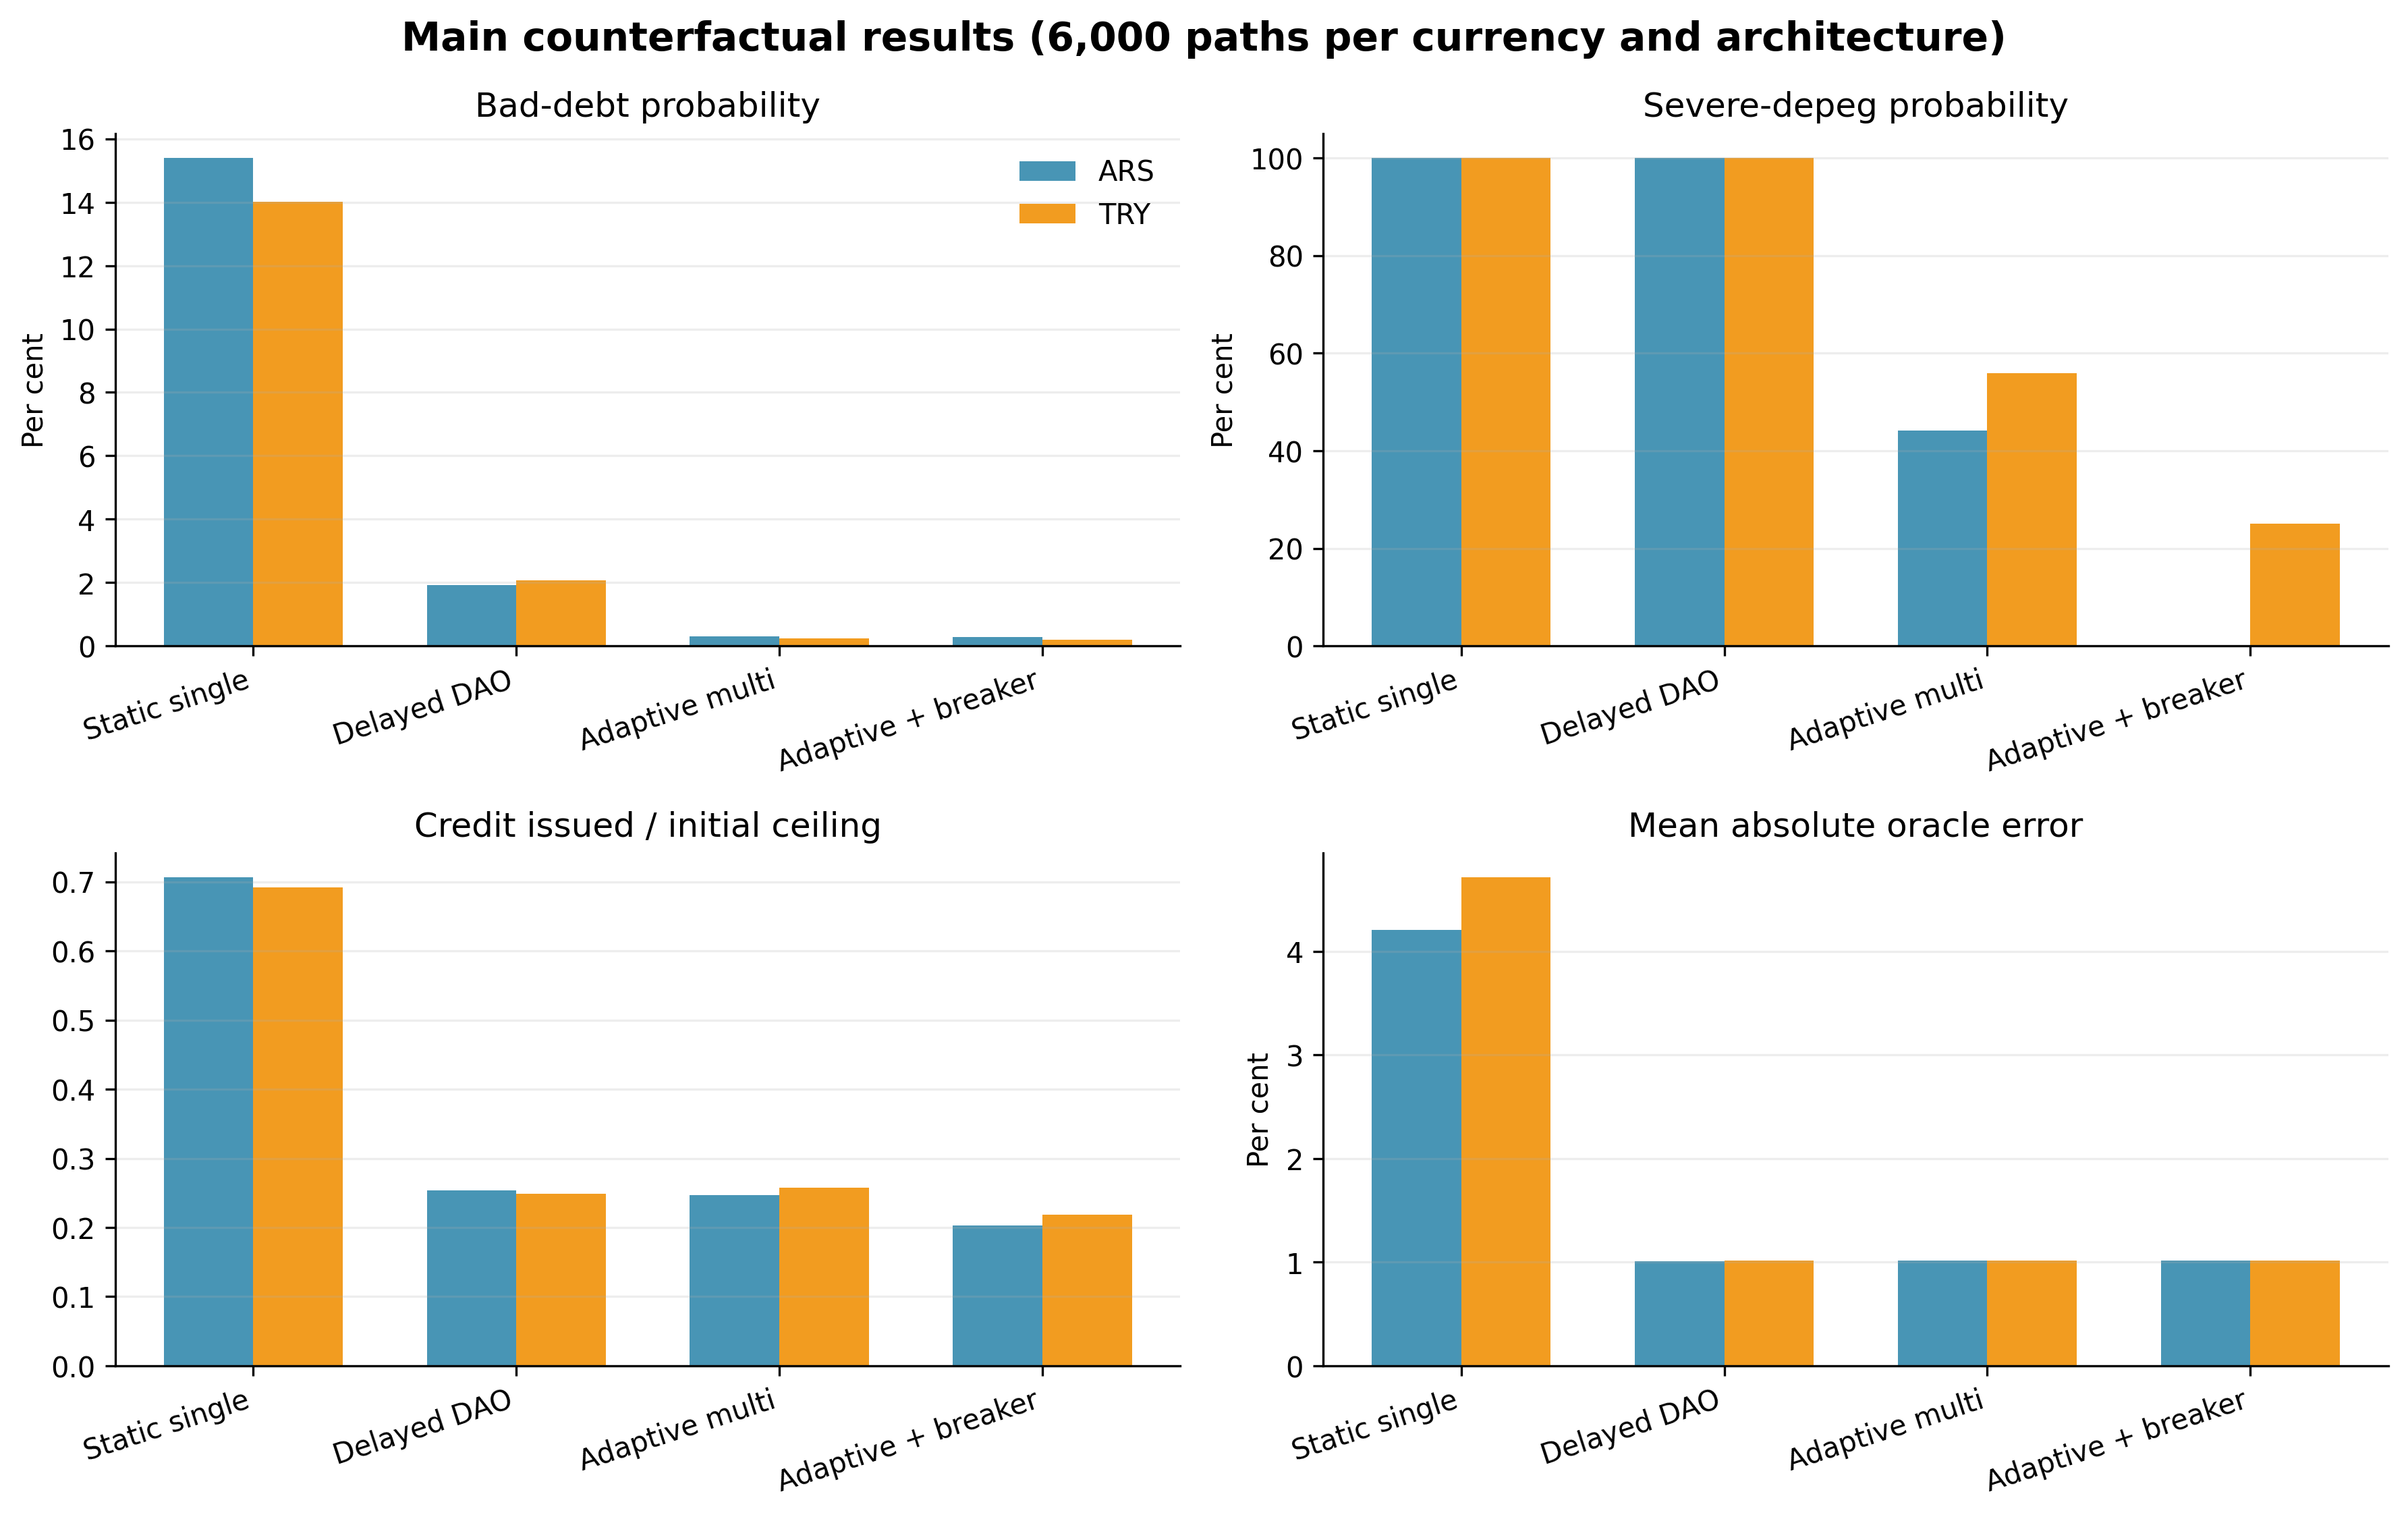
\includegraphics[width=\textwidth]{../figures/figure3_main_outcomes.png}
\caption{Main counterfactual outcomes. Bars report the 6,000-path mean or event probability for each currency-architecture cell.}
\label{fig:main}
\end{figure*}

Bad-debt prevention and peg support are not the same result. Every static and delayed-DAO path crosses the 10\% severe-depeg threshold. Immediate adaptive controls reduce the probability to 44.2\% for ARS and 55.9\% for TRY by pricing and limiting new issuance. The breaker reduces it to zero for ARS and 25.0\% for TRY. The remaining TRY events occur on paths where a large within-month FX move raises background conversion flow above correction capacity even after new protocol borrowing is stopped.

The cost appears in the same table. Static cumulative credit is 0.706 initial-ceiling units for ARS and 0.692 for TRY. The full architecture supplies 0.203 and 0.218. The breaker is active for 28.0\% and 29.1\% of intervals. Mean annualised borrowing rates rise to 61.4\% and 64.3\%, while mean ceilings fall to 0.439 and 0.437. These are stress-policy outputs, not recommended user prices. They show that safety is obtained partly by withdrawing the protocol's balance sheet.

\subsection{Oracle accuracy and liquidation quality}

Mean oracle error falls from 4.20\% (ARS) and 4.71\% (TRY) under the static composite to about 1.01\% under each multi-source architecture. Table~\ref{tab:oracle} also reports the upper tail and liquidation outcomes. The P95 maximum error remains large---approximately 37\%---even for the median architecture because a discontinuous collateral move can leave two of three sources temporarily stale. Medianization is robust to one bad source, not to correlated latency.

\begin{table*}[t]
\centering
\caption{Oracle, liquidation, and controller outcomes.}\label{tab:oracle}
\small
\setlength{\tabcolsep}{4pt}
\begin{tabular}{llrrrrr}
\toprule
Currency & Architecture & P95 max error & Liquidations & Unnecessary & Mean rate & Mean ceiling \\
\midrule
ARS & Static single & 30.61\% & 9.91 & 0.47 & 8.0\% & 1.000 \\
ARS & Delayed DAO & 36.98\% & 36.19 & 0.00 & 67.7\% & 0.447 \\
ARS & Adaptive multi & 36.98\% & 57.51 & 0.01 & 67.9\% & 0.402 \\
ARS & Adaptive + breaker & 36.98\% & 57.91 & 0.01 & 61.4\% & 0.439 \\
TRY & Static single & 37.33\% & 9.52 & 1.42 & 8.0\% & 1.000 \\
TRY & Delayed DAO & 37.09\% & 32.99 & 0.03 & 69.4\% & 0.450 \\
TRY & Adaptive multi & 37.09\% & 46.58 & 0.05 & 68.3\% & 0.414 \\
TRY & Adaptive + breaker & 37.09\% & 45.18 & 0.03 & 64.3\% & 0.437 \\
\bottomrule
\end{tabular}

\end{table*}

Figure~\ref{fig:latency} shows why an official rate can be operationally conservative yet costly. Increasing the official--parallel gap raises unnecessary liquidations strongly; at twice the baseline gap, the pooled mean exceeds four events per path. Longer latency compounds the effect. Mean oracle error rises from approximately 0.1\% with no gap and no delay to 8.9\% at the largest gap and 48-hour delay. Bad-debt probability is less monotone in this grid because an official rate that values the local currency above its executable price increases the observed debt value and can cause earlier, conservative liquidation. The architecture must therefore evaluate both lender loss and borrower liquidation cost.

\begin{figure*}[t]
\centering
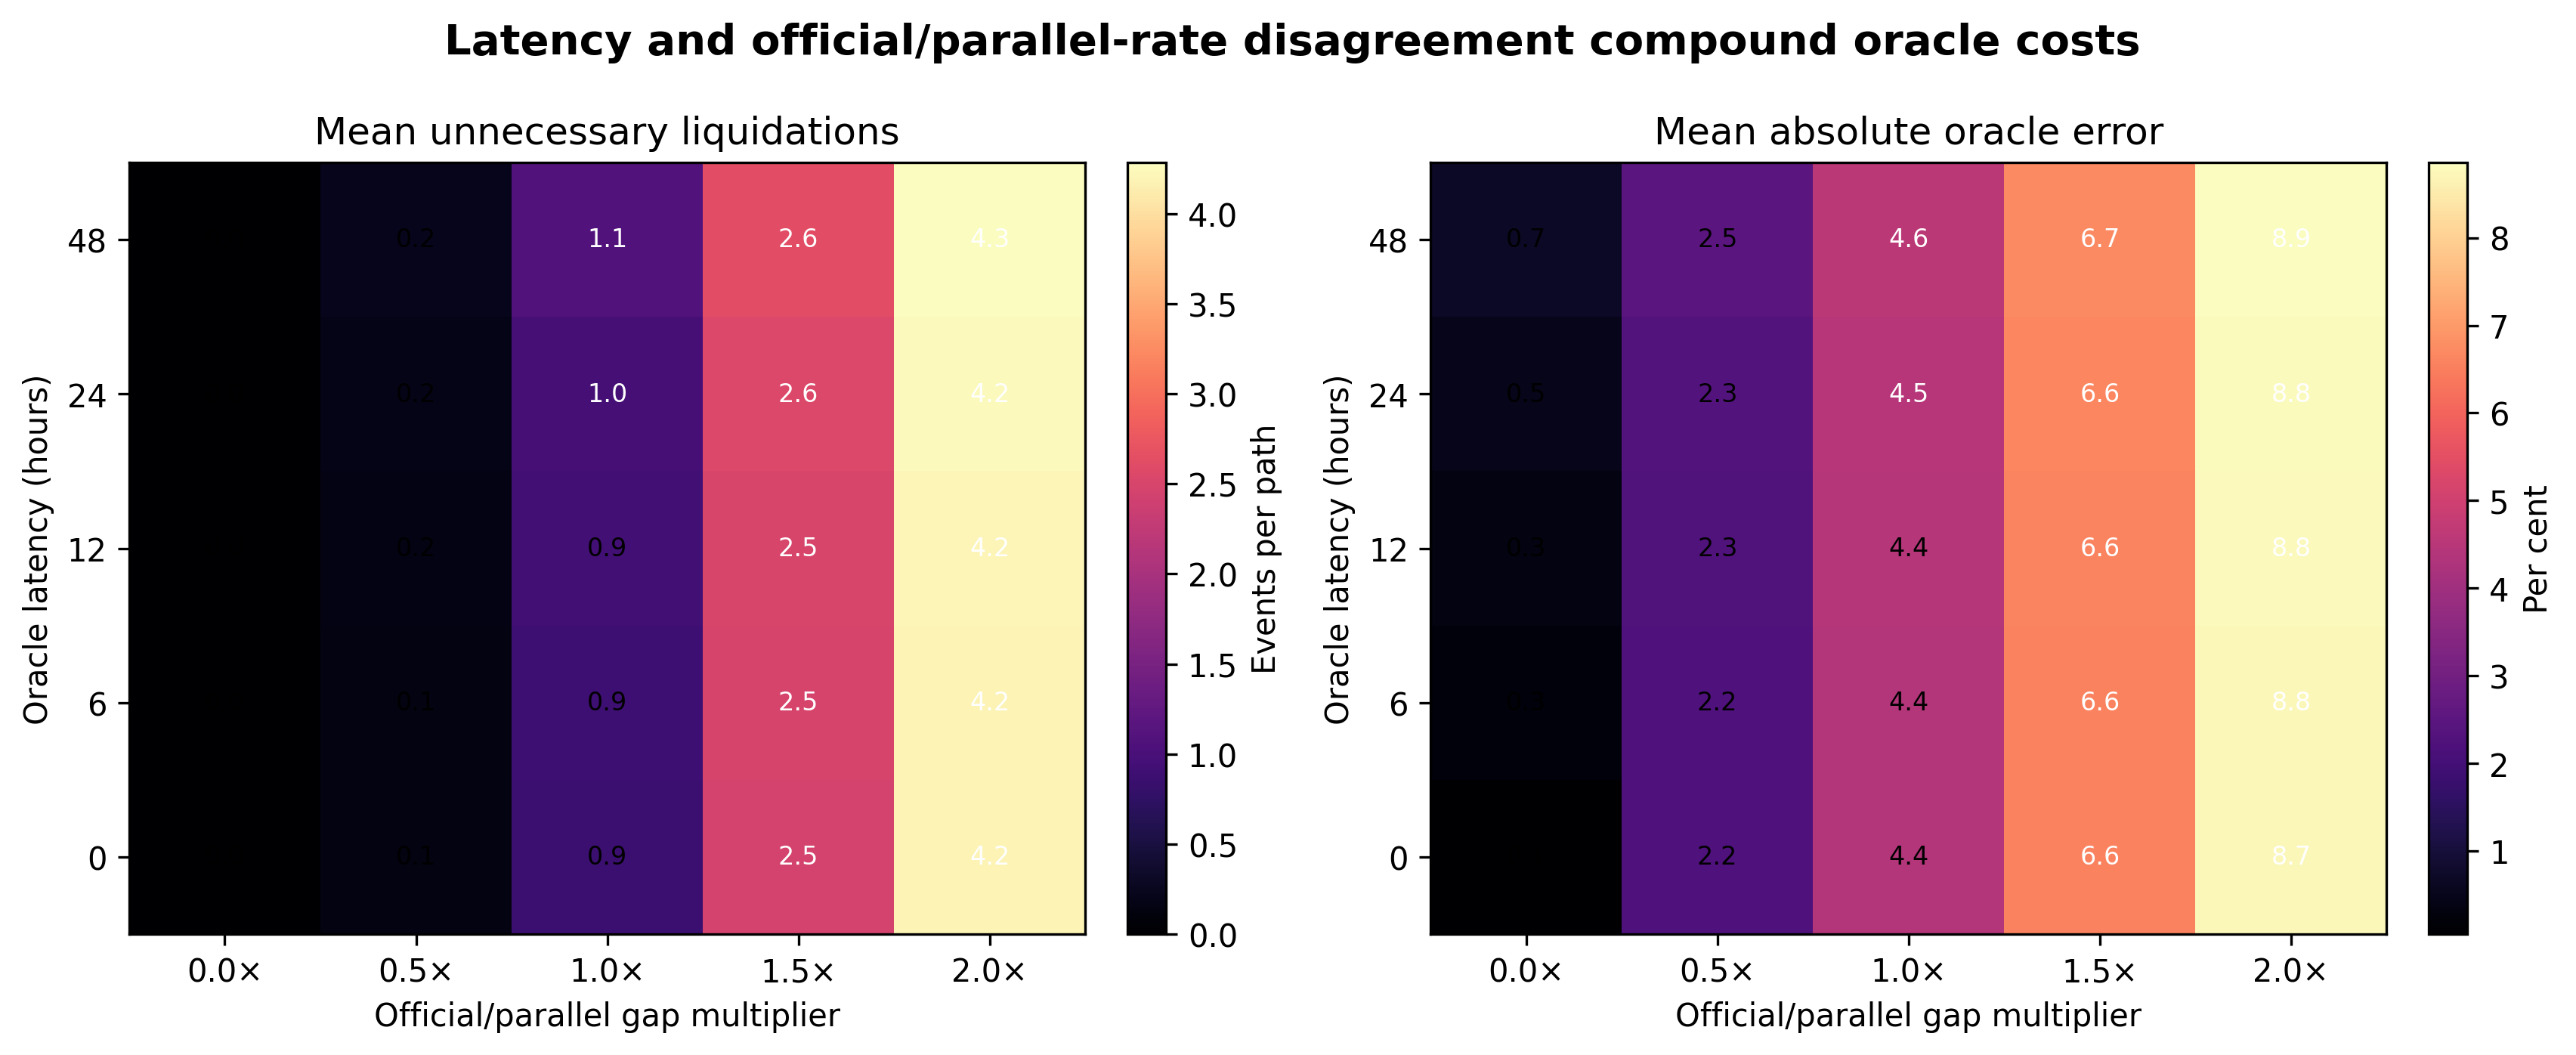
\includegraphics[width=\textwidth]{../figures/figure4_latency_basis_heatmap.png}
\caption{Pooled latency--basis sensitivity for the static architecture. The left panel reports unnecessary liquidation events per path; the right reports mean absolute oracle error.}
\label{fig:latency}
\end{figure*}

\subsection{One-source manipulation}

Figure~\ref{fig:attack} varies the four-step DEX collateral attack. With no attack, pooled static bad-debt probability is 14.4\%; at the baseline attack it is 16.0\%, and at twice baseline it is 20.4\%. P95 maximum oracle error rises from 24.7\% to 64.2\%. The full architecture's bad-debt probability remains 0.33\% and its corresponding error statistic is unchanged across attack scales because the manipulated source does not move the median. This result depends on source independence. If two feeds share a venue, data provider, bridge, or signer set, a nominal three-source median may have only one or two effective sources.

\begin{figure*}[t]
\centering
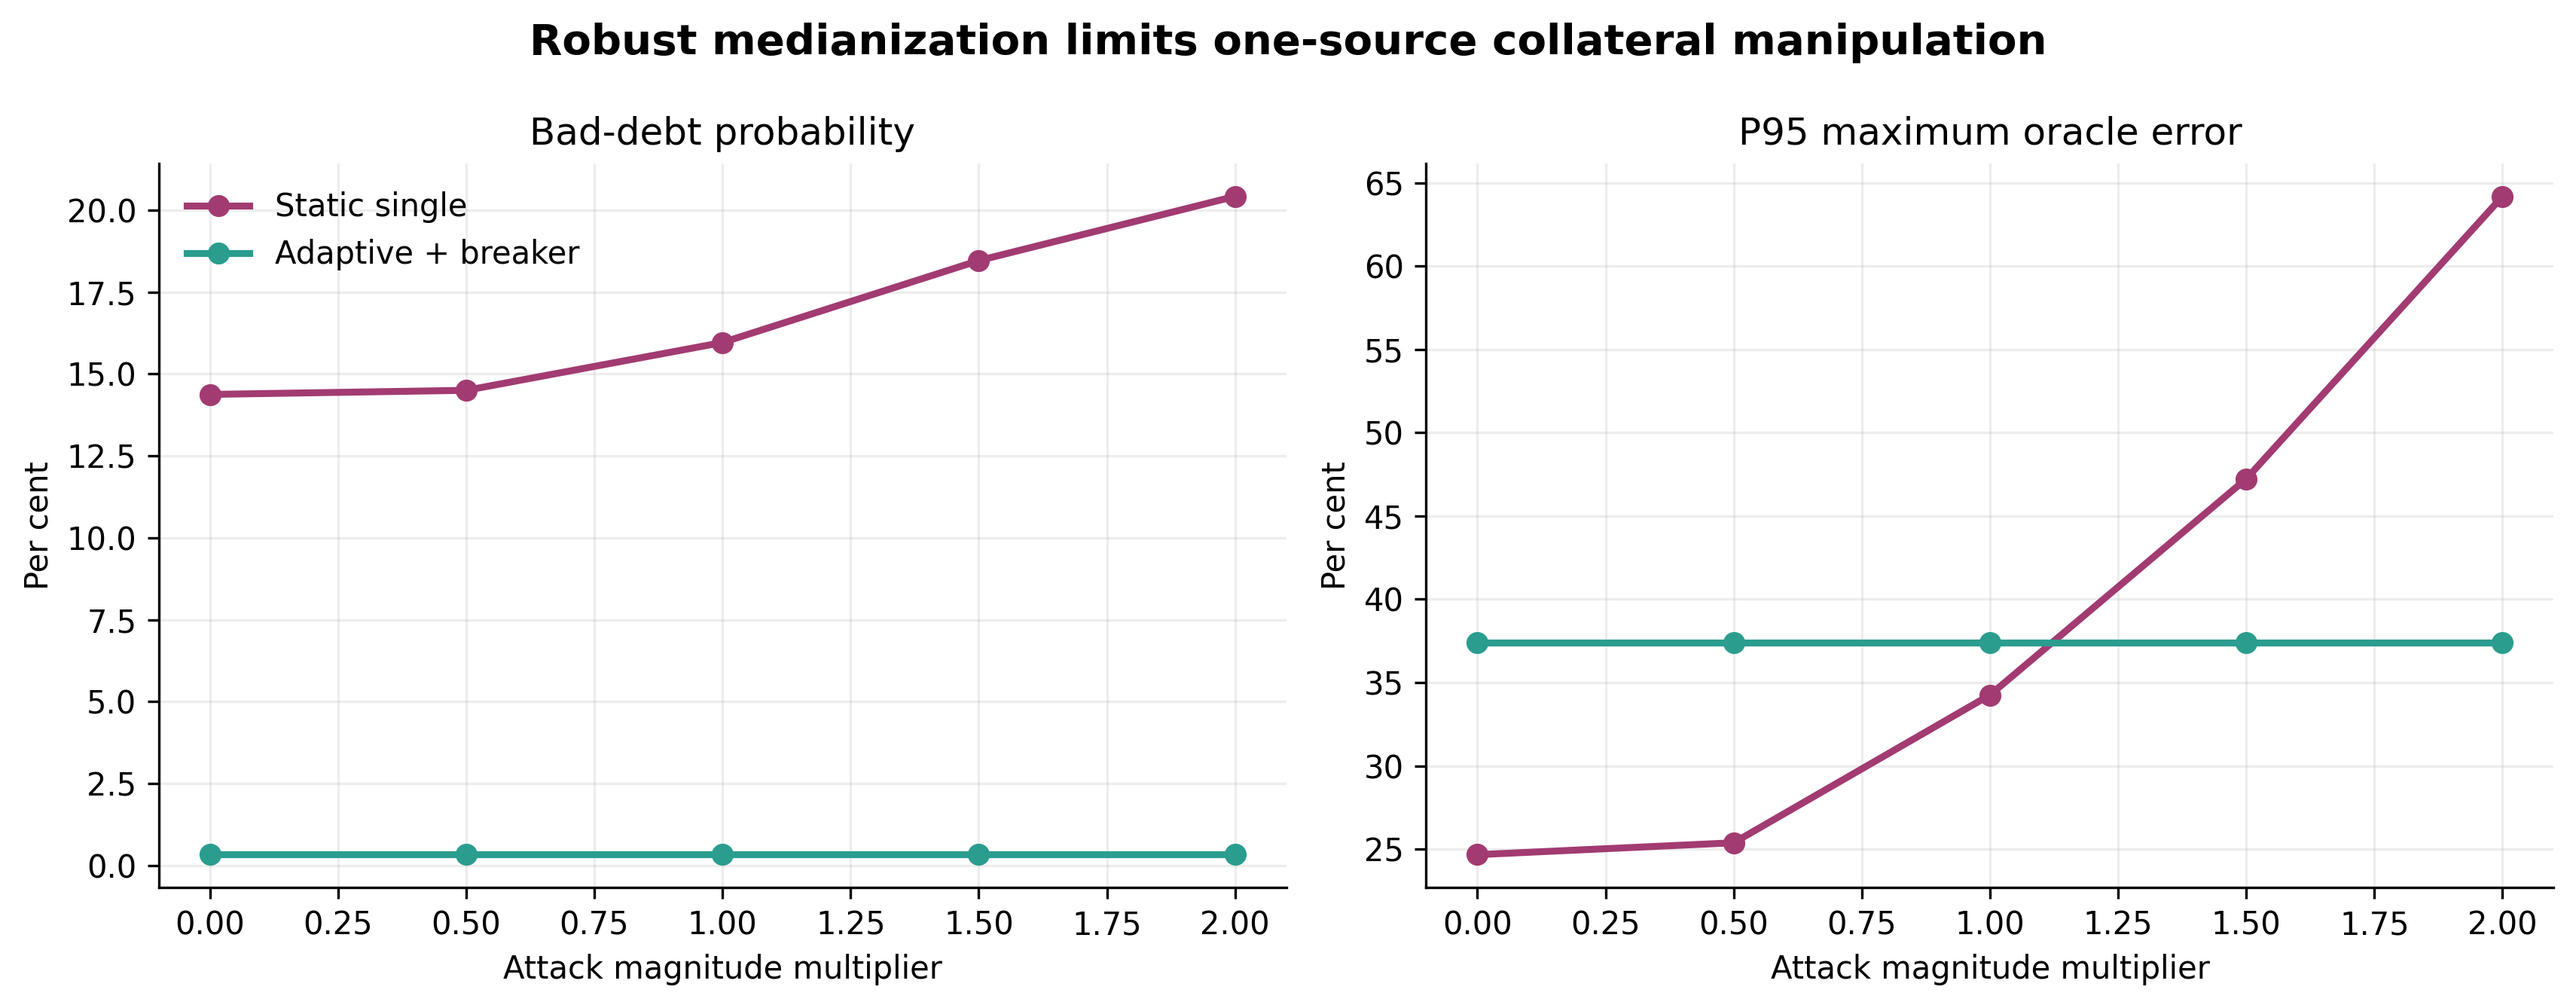
\includegraphics[width=\textwidth]{../figures/figure5_attack_robustness.png}
\caption{Attack-magnitude sensitivity pooled across currencies. The robust architecture rejects the single manipulated collateral source; the static benchmark admits opportunistic borrowing against that source.}
\label{fig:attack}
\end{figure*}

\subsection{Governance delay}

Delay removes the controller's advantage quickly (Figure~\ref{fig:delay} and Table~\ref{tab:delay}). With immediate execution and no breaker, severe-depeg probability in the sensitivity sample is 45.1\% for ARS and 55.8\% for TRY. At 12 hours these values rise to 57.6\% and 65.3\%. At 24 hours ARS reaches 100\% and TRY 88.0\%; at 48 hours both are 100\%. Bad-debt probability also rises monotonically after short delays, reaching 2.25\% and 2.75\% at 48 hours and 2.67\% and 3.50\% at 72 hours.

\begin{figure*}[t]
\centering
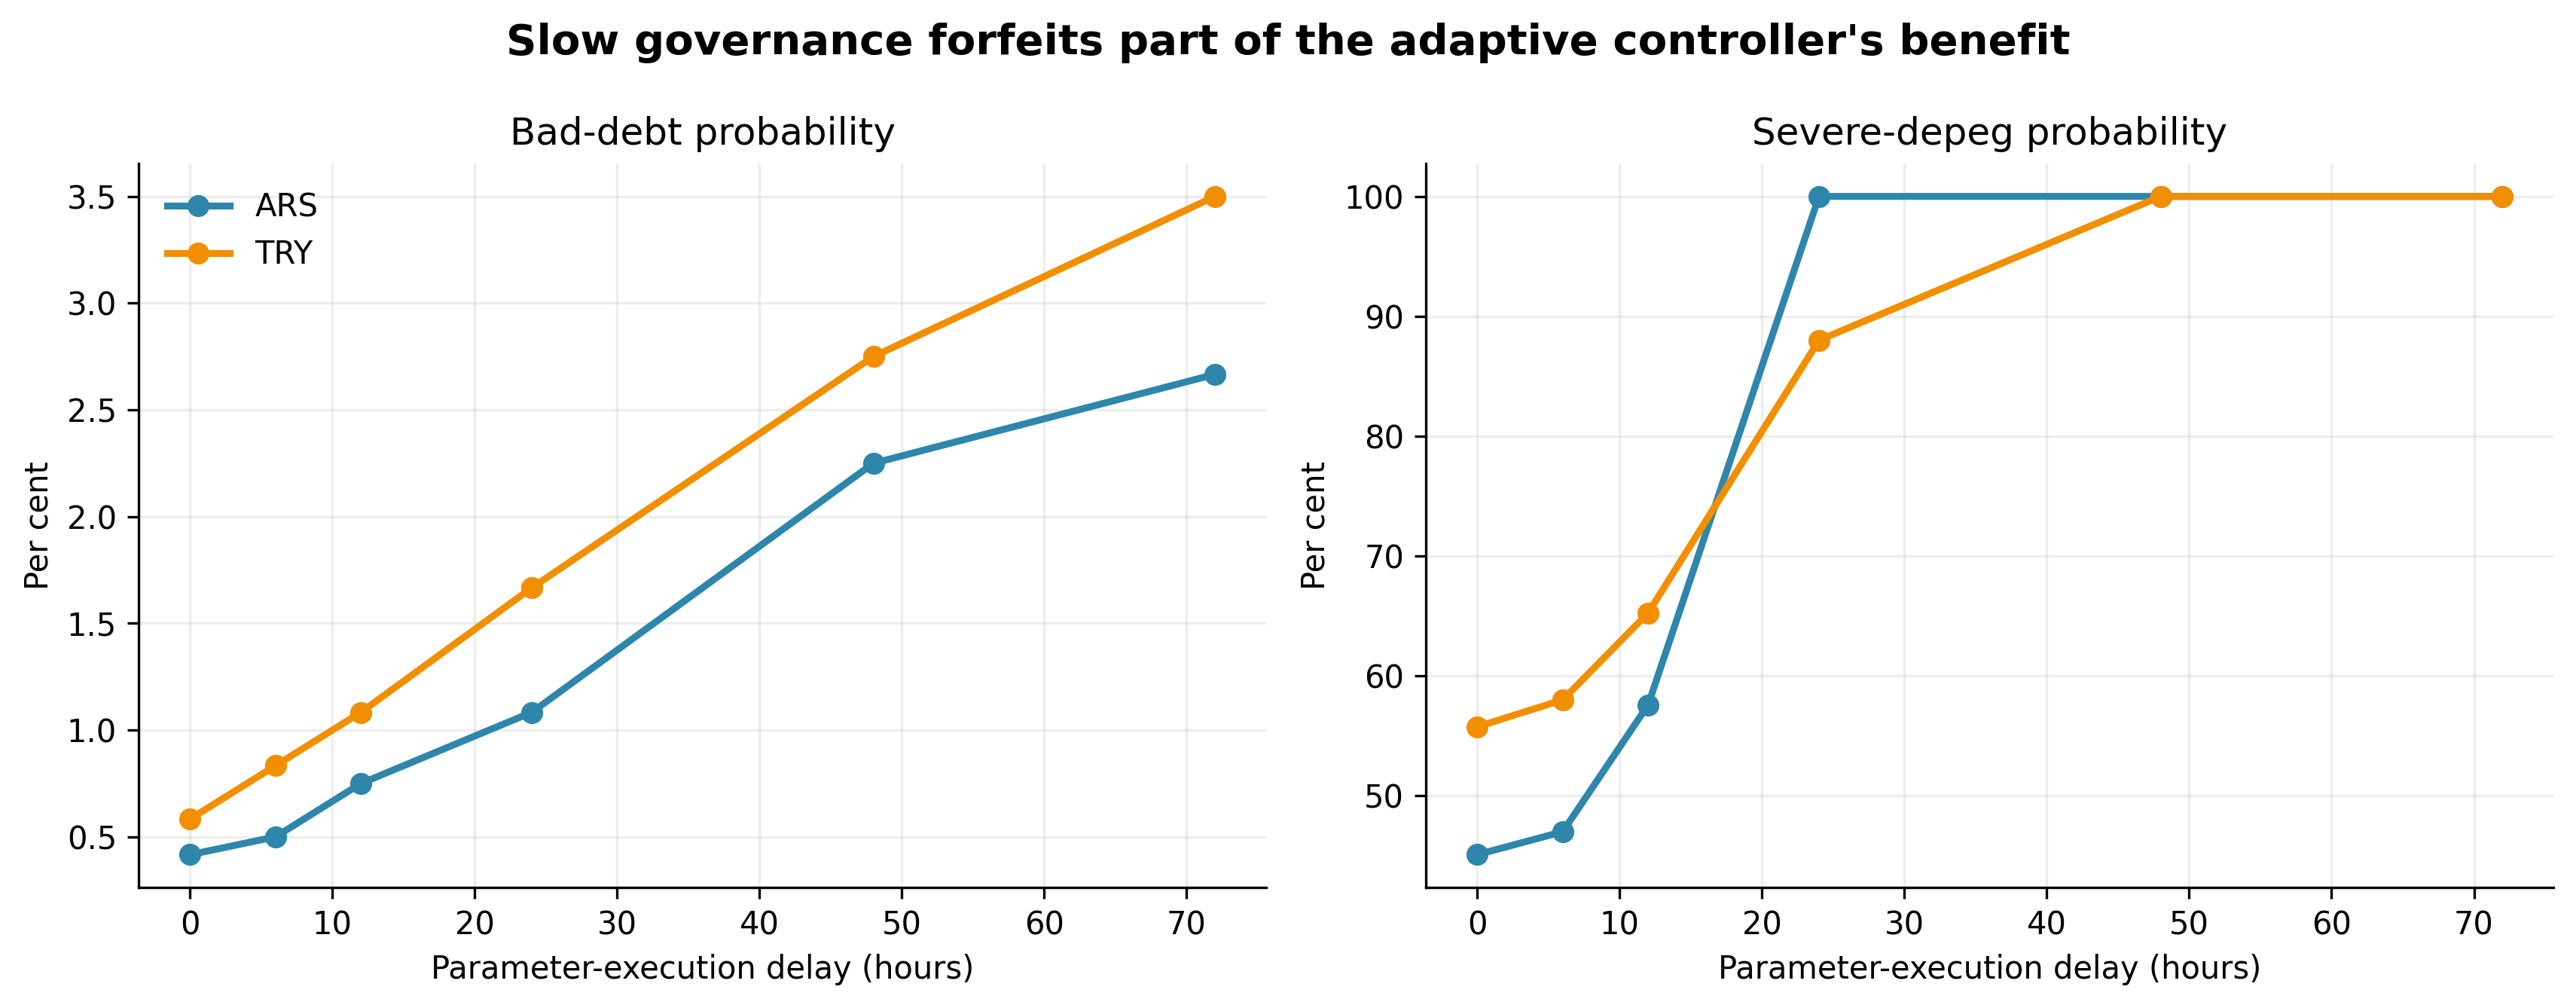
\includegraphics[width=\textwidth]{../figures/figure6_governance_delay.png}
\caption{Effect of parameter-execution delay on the adaptive multi-oracle architecture without a breaker.}
\label{fig:delay}
\end{figure*}

\begin{table*}[t]
\centering
\caption{Governance-delay sensitivity.}\label{tab:delay}
\small
\begin{tabular}{lrrrrr}
\toprule
Delay & ARS bad debt & TRY bad debt & ARS depeg & TRY depeg & Mean credit \\
\midrule
0 h & 0.4\% & 0.6\% & 45.1\% & 55.8\% & 0.254 \\
6 h & 0.5\% & 0.8\% & 47.0\% & 58.0\% & 0.253 \\
12 h & 0.8\% & 1.1\% & 57.6\% & 65.2\% & 0.250 \\
24 h & 1.1\% & 1.7\% & 100.0\% & 88.0\% & 0.247 \\
48 h & 2.2\% & 2.8\% & 100.0\% & 100.0\% & 0.252 \\
72 h & 2.7\% & 3.5\% & 100.0\% & 100.0\% & 0.268 \\
\bottomrule
\end{tabular}

\end{table*}

The nonlinearity is important. A vote that is only one day late is not simply one day less optimal. If issuance continues while basis persistence and market impact operate, the controller begins from a worse state when it finally acts. This is a case for pre-authorised bounded actions and an emergency stop, not for removing human governance. Structural parameters, code upgrades, risk-score weights, source admission, and controller renewal remain governance decisions.

\subsection{Controller ablation}

Table~\ref{tab:ablation} identifies which instruments drive which outcome. A rate-only design retains the unit ceiling and leaves pooled bad-debt probability near 9\%; it reduces but does not eliminate severe depeg. A ceiling-only design reduces credit to about 0.118 but leaves bad-debt probability near 8\% because it does not raise collateral protection. A liquidation-only design makes bad debt rare but admits about 0.87 unit of new credit and produces a severe depeg in every path. All three continuous controls are needed for the combined objective. The breaker adds the hard bound on endogenous issuance during extreme states, reducing pooled severe-depeg probability from about 50.6\% to 11.6\%, at a pause share near 28.9\%.

\begin{table*}[t]
\centering
\caption{Controller ablation, pooled equally across ARS and TRY.}\label{tab:ablation}
\small
\begin{tabular}{lrrrrr}
\toprule
Design & Bad debt & Severe depeg & Credit & Pause & Mean ceiling \\
\midrule
Rate only & 9.2\% & 58.9\% & 0.304 & 0.0\% & 1.000 \\
Ceiling only & 8.0\% & 100.0\% & 0.118 & 0.0\% & 0.233 \\
Liquidation only & 0.5\% & 100.0\% & 0.872 & 0.0\% & 1.000 \\
All controls & 0.2\% & 50.6\% & 0.256 & 0.0\% & 0.411 \\
All + breaker & 0.2\% & 11.6\% & 0.213 & 28.9\% & 0.441 \\
\bottomrule
\end{tabular}

\end{table*}

\subsection{Historical replay and representative path}

The 39 realised windows support the qualitative ranking. Static bad-debt frequency is 15.4\% for ARS and 12.8\% for TRY. No multi-oracle architecture records a material bad-debt event in these small realised-window samples, although they are not independent trials. Static and delayed-DAO designs depeg in every realised window. The full architecture records zero severe ARS depegs and seven of 39 TRY depegs (17.9\%).

Figure~\ref{fig:path} follows the most adverse joint ARS/ETH macro path placed deterministically at path zero. The static oracle carries a persistent negative ratio error, credit grows almost linearly, and the DEX discount settles near 25\%. The full architecture raises the rate and liquidation buffer, reduces the ceiling, and repeatedly pauses new draws. Its discount remains near the breaker boundary and cumulative credit is roughly one quarter of the static path. Temporary oracle-error spikes remain visible, reinforcing that medianization is not instantaneous truth.

\begin{figure*}[t]
\centering
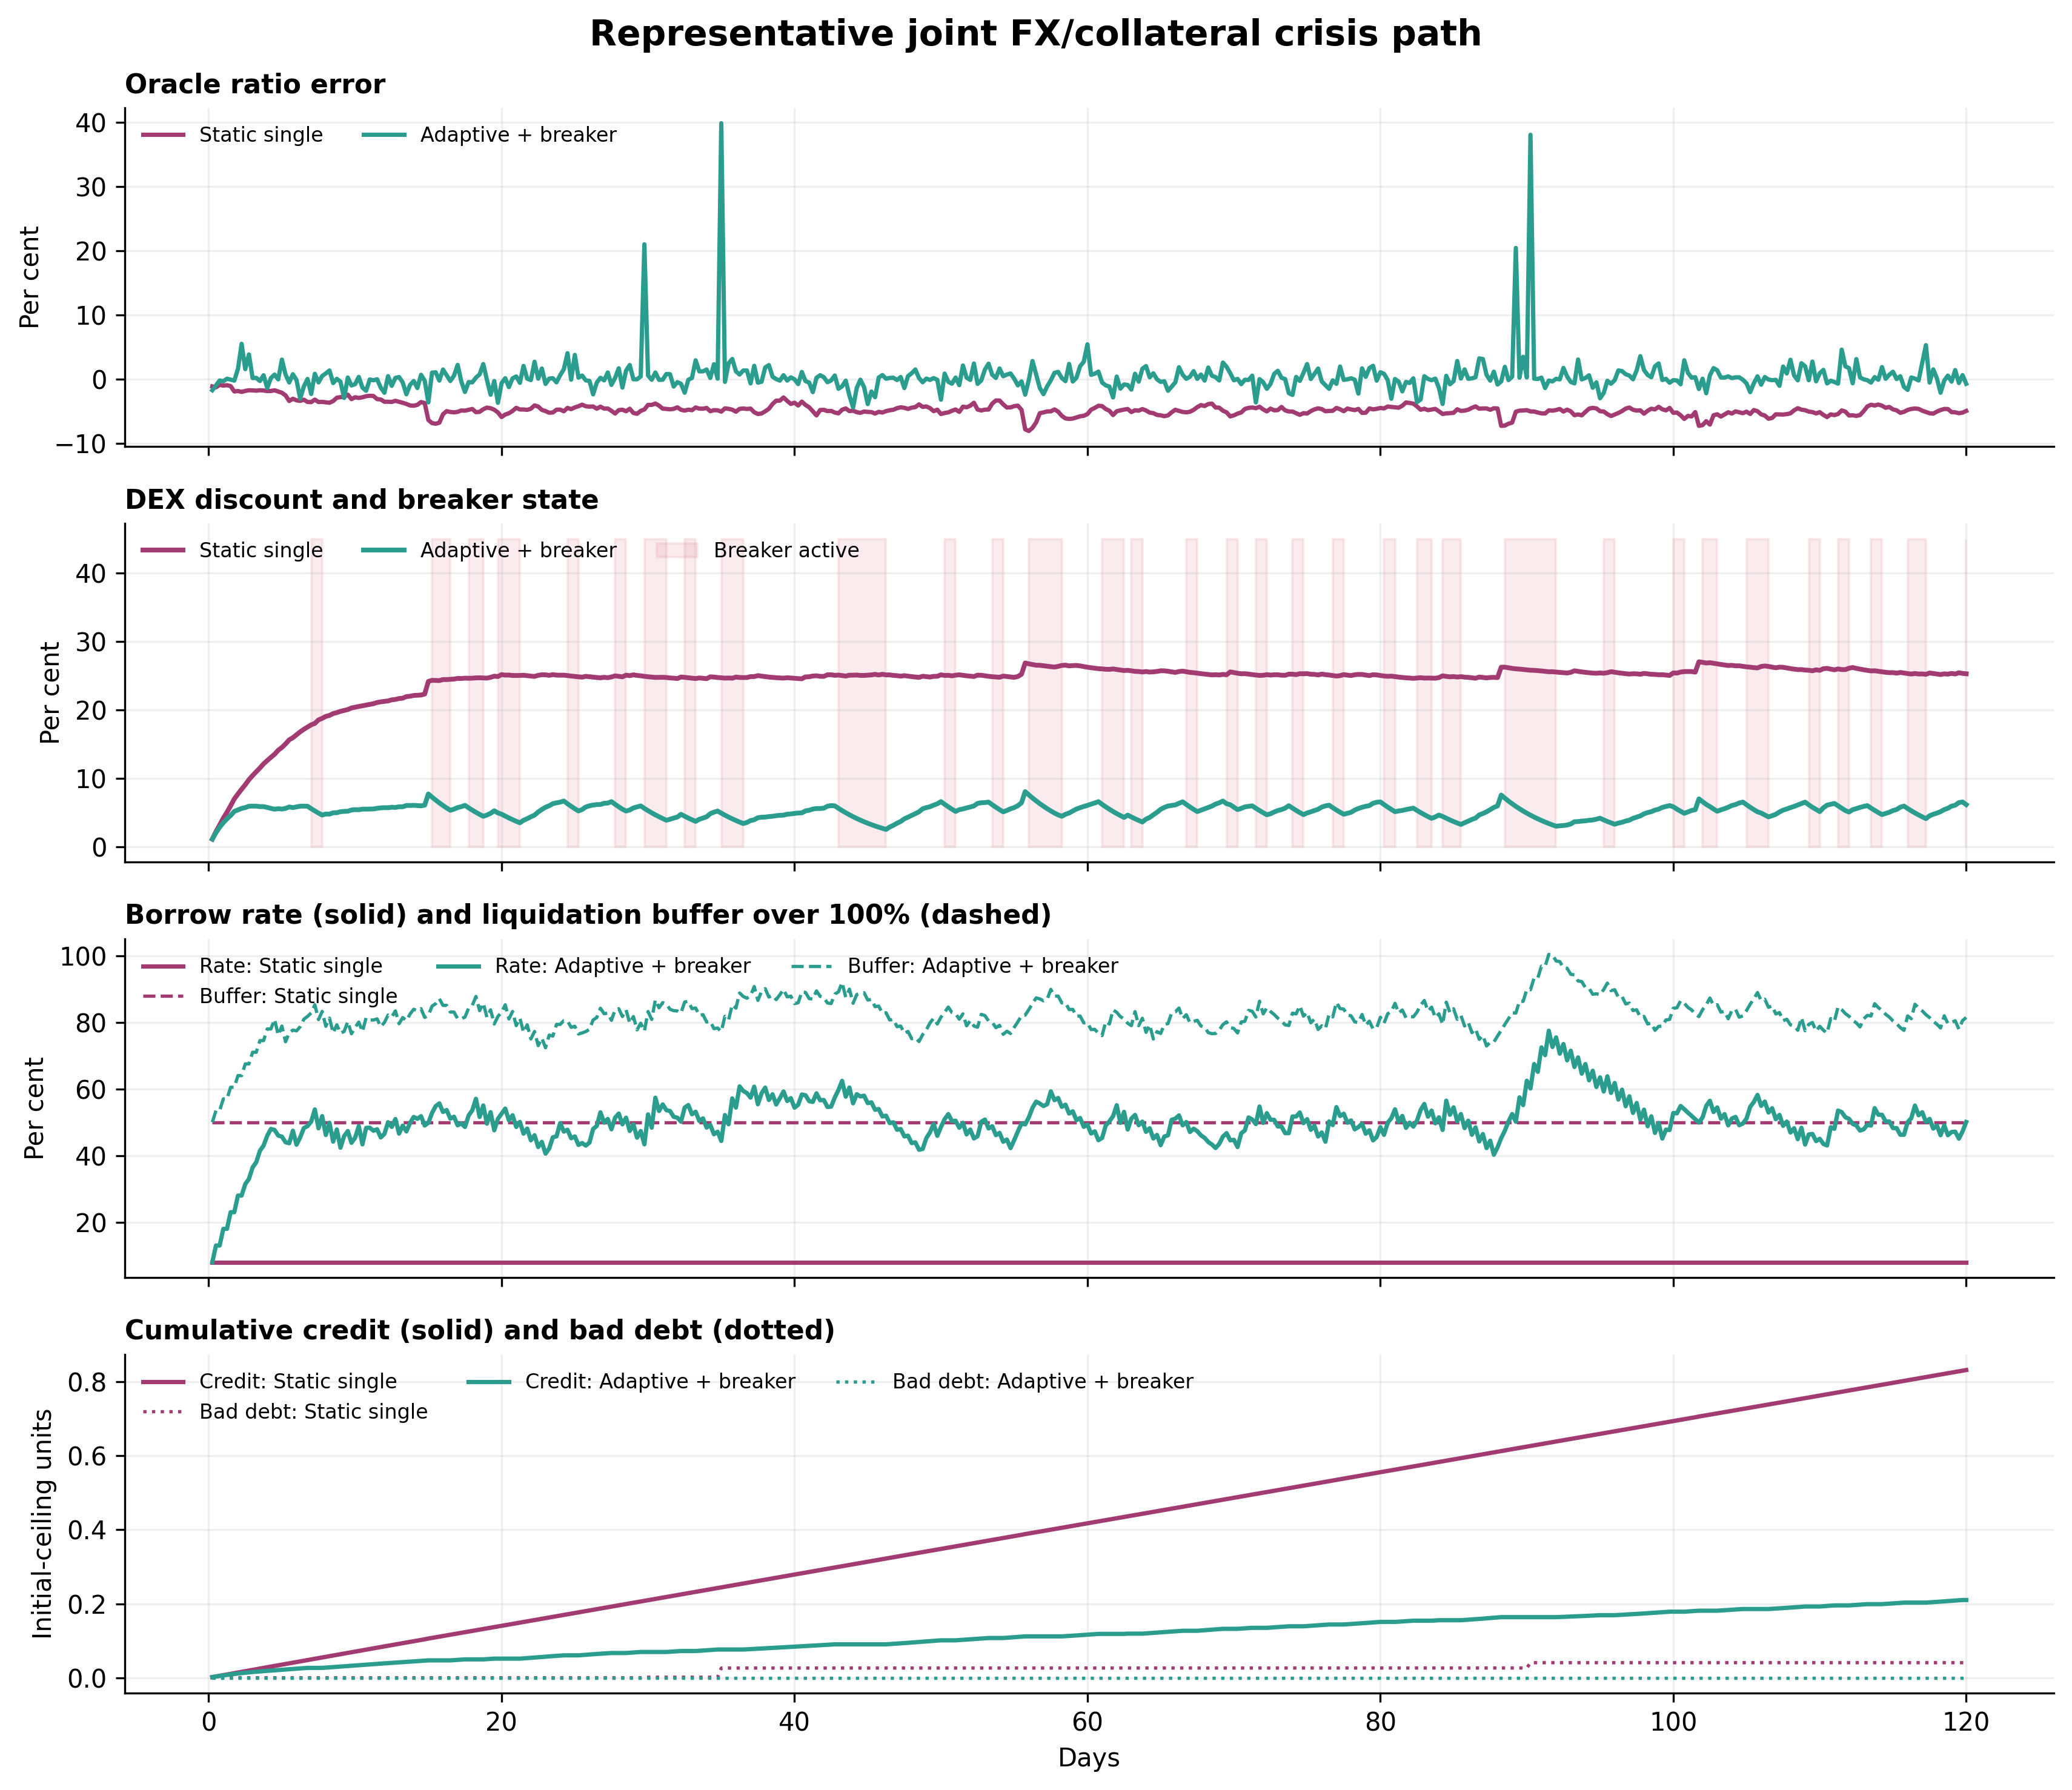
\includegraphics[width=\textwidth]{../figures/figure7_representative_crisis_path.png}
\caption{Representative joint FX/collateral crisis path. Red shading indicates intervals in which the full architecture's breaker is active.}
\label{fig:path}
\end{figure*}

\section{Implementation and Governance Blueprint}\label{sec:blueprint}

The simulation suggests a separation of authority rather than fully autonomous governance.

\subsection{On-chain bounded mandate}

Governance can authorise a controller contract to move only three named parameters inside hard domains and per-interval limits. The source set, score coefficients, breaker thresholds, cooldown, and action bounds should be immutable for an epoch or change only through the ordinary delayed governance path. This converts automation from unlimited discretion into a narrow mandate.

Every update should emit the source values, timestamps, disagreement, risk score, old parameters, target parameters, applied bounded action, and trigger flags. Reproducing an action should require no private model state. A controller that cannot be independently replayed undermines the transparency advantage of DeFi.

\subsection{Oracle independence and fallback}

Source diversity should be measured by failure domain, not brand count. Two feeds derived from the same thin pool or off-chain vendor are not independent. The protocol should document venue, aggregation window, signer or reporter set, bridge dependence, quote currency, update trigger, heartbeat, and legal/settlement meaning for each source.

Fallback should be state dependent. A stale source need not be replaced by the latest manipulable trade. The safe response may be to exclude the source from new borrowing, use a conservative price for exposure increases, retain a separate liquidation guard, and activate the breaker when the remaining quorum is insufficient. The exact rule must avoid allowing an attacker to force liquidations merely by making sources disagree.

\subsection{Human override and renewal}

An emergency role should be able to make the system more restrictive---pause new borrowing or lower an exposure cap---but not silently increase risk. Relaxation should follow ordinary governance. The controller mandate should expire unless renewed after evaluation against new market data, attack simulations, and realised false-positive rates. This creates accountability without requiring a token vote for each six-hour risk update.

\section{Discussion}\label{sec:discussion}

\subsection{What the results establish}

Within the stated model, three claims are supported. First, a robust multi-source price layer materially reduces the effect of one-source collateral manipulation and average cross-domain error. Second, coordinating rate, ceiling, and liquidation controls is more effective than relying on any one parameter. Third, a hard pause on new draws can prevent protocol-originated issuance from amplifying a depeg when continuous controls respond too slowly.

The paired-path design makes these architecture comparisons precise for the simulation. It does not identify causal effects in live market data. Event probabilities are conditional on the return resampling, bridge, demand, attack, depth, arbitrage, haircut, and controller assumptions.

\subsection{Why TRY risk remains}

The full architecture does not force a zero TRY severe-depeg rate. TRY monthly depreciation has a much larger observed upper tail than ARS in the common window (26.8\% versus 7.6\%). Assigning part of that move to a six-hour interval can create conversion flow beyond the modelled correction capacity before or independently of new borrowing. Once new draws are zero, the protocol has exhausted the control represented here.

This boundary links the third and fourth papers. Peg support requires liquidity, arbitrage capital, and settlement access; governance controls the protocol's contribution to flow but not the external balance sheet. A production design would therefore need explicit reserves, redemption capacity, market-maker commitments, or a different issuance promise. Adding those resources would change the economic model and should not be described as a software-only improvement.

\subsection{Borrower protection}

The loss numbers alone would favour aggressive controls. Borrowers experience a different objective: high rates, reduced ceilings, more liquidations, and long pause time. The full architecture's approximately 28--29\% pause share is large. This is not a hidden implementation inconvenience; it is the measured price of the chosen breaker thresholds.

A production policy should publish service-level objectives for maximum pause time, appeal or compensation processes for oracle-caused liquidation, and the conditions for reopening. The protocol should also distinguish existing positions from new exposure. Allowing repayment and collateral addition during a pause is the minimum asymmetric protection considered here.

\section{Limitations}\label{sec:limitations}

The study has eight material limitations. First, the calibration window contains only 42 monthly joint returns and two currencies. Block sampling preserves short dependence but cannot create unobserved regimes. Second, six-hour paths are synthetic bridges constrained to observed monthly endpoints; intramonth volatility and jump timing are scenario assumptions. Third, the official--parallel gap is modelled rather than sourced from a harmonised historical series. Fourth, DEX basis uses a reduced-form depth and capacity equation, not a full order book, concentrated-liquidity AMM, or cross-venue network.

Fifth, borrower demand is elastic and opportunistic by construction; it is not estimated from a live local-currency protocol. Sixth, liquidation occurs mechanically at an endogenous haircut without gas congestion, liquidator competition, MEV, or chain reorganisation. Seventh, source failures are simplified to one manipulated DEX collateral feed; correlated reporter, bridge, governance, and stablecoin-reserve failures could defeat the median. Eighth, the controller weights and thresholds are transparent engineering choices, not optimal-control estimates or formally verified safety bounds.

The model also excludes legal restrictions, sanctions, capital-control enforcement, banking cut-off times, reserve custody, smart-contract bugs, governance-token concentration, voter participation, and attacks on the controller itself. These omissions prevent interpreting the results as a deployment approval. The correct next empirical step is to calibrate source-specific latency and basis dynamics from timestamped official, exchange, and DEX data and evaluate the controller in a shadow mode before any on-chain authority is granted.

\section{Conclusion}\label{sec:conclusion}

A local-currency DeFi lending protocol cannot treat governance, oracles, and market liquidity as separate layers. The price used to admit debt changes the collateral users must post; debt issuance changes DEX flow; the DEX basis changes protocol risk; and a delayed governance response acts on a state partly created during its own delay.

The proposed architecture combines three price domains, a disagreement-aware risk state, bounded controls for the borrowing rate, debt ceiling, and liquidation ratio, and an asymmetric circuit breaker. In the reproducible counterfactual, it reduces bad-debt probability from roughly 14--15\% to approximately 0.2--0.3\%. It eliminates severe ARS depegs in the main experiment and reduces, but does not eliminate, TRY depegs. The improvement consumes credit availability and pauses new borrowing in nearly three of every ten intervals.

The central design conclusion is therefore not ``automate governance.'' It is more specific: pre-authorise narrow, monotone, rate-limited defensive actions; aggregate genuinely independent price sources; treat freshness and economic disagreement as separate risks; preserve deleveraging during emergencies; and disclose the credit cost of safety. Human governance should define and renew that mandate. Market makers and settlement capacity must support it. No controller can substitute for both.

\section*{Data Availability}

The replication package contains the original FRED/OECD ARS and TRY CSV snapshots, the common processed monthly FX/crypto panel, SHA-256 checksums, and every generated result file. The Coin Metrics ETH series is included in the processed panel inherited from the companion solvency repository. No proprietary dataset, private wallet, or paid API is required. Source identifiers, URLs, transformations, and licensing notes are recorded in \texttt{documentation/SOURCES.md}.

\section*{Code Availability}

Python code constructs the joint block samples, exact monthly bridges, oracle feeds, lending book, adaptive controller, circuit breaker, robustness exercises, figures, LaTeX tables, and validation anchors. A pinned requirements file, deterministic seed, unit tests, and \texttt{run\_all.sh} reproduce the complete paper with one command. The repository is available at \url{https://github.com/nikorokni/local-currency-defi-adaptive-governance}.

\section*{Author Contributions}

Niko Rokni Lamouki: Conceptualization, Methodology, Software, Formal analysis, Data curation, Visualization, Writing---original draft, Writing---review and editing, Project administration. Salma Soofiyan: Validation, Investigation, Writing---review and editing.

\section*{Declarations}

\textbf{Funding.} No external funding was reported for this study.\\
\textbf{Competing interests.} The authors declare no competing interests.\\
\textbf{Ethics approval.} Not applicable; the study uses public aggregate market data and simulation.\\
\textbf{Consent to participate.} Not applicable.\\
\textbf{Consent for publication.} Not applicable.

\begin{thebibliography}{99}

\bibitem{RokniLamouki2026Debt}
Rokni Lamouki N, Soofiyan S.
Inflation-driven debt erosion in local-currency DeFi lending: Counterfactual evidence from MakerDAO ETH-A borrowing activity.
Working paper and replication package. 2026.
Available from: \url{https://github.com/nikorokni/inflation-driven-debt-erosion-defi}.

\bibitem{RokniLamouki2026Solvency}
Rokni Lamouki N, Soofiyan S.
From debt erosion to protocol solvency: Path-dependent stress testing of local-currency DeFi lending under joint FX and crypto-collateral shocks.
Working paper and replication package. 2026.
Available from: \url{https://github.com/nikorokni/local-currency-defi-solvency-stress-test}.

\bibitem{RokniLamouki2026Peg}
Rokni Lamouki N, Soofiyan S.
From debt erosion to peg stability: Liquidity provision, arbitrage bottlenecks, and secondary market dynamics for local-currency DeFi stablecoins.
Working paper and replication package. 2026.
Available from: \url{https://github.com/nikorokni/local-currency-defi-peg-stability}.

\bibitem{Eskandari2021}
Eskandari S, Salehi M, Gu WC, Clark J.
SoK: Oracles from the ground truth to market manipulation.
arXiv:2106.00667. 2021.
doi:10.48550/arXiv.2106.00667.

\bibitem{Qin2021}
Qin K, Zhou L, Livshits B, Gervais A.
Attacking the DeFi ecosystem with flash loans for fun and profit.
In: \textit{Financial Cryptography and Data Security}. 2021. pp. 3--32.
doi:10.1007/978-3-662-64322-8\_1.

\bibitem{Bai2025}
Bai D, Cao J, Cao Y, Wen L.
Ormer: A manipulation-resistant and gas-efficient blockchain pricing oracle for DeFi.
arXiv:2410.07893. 2025.
doi:10.48550/arXiv.2410.07893.

\bibitem{Sadeghi2026}
Sadeghi A, Feinstein Z.
Liquidation dynamics in DeFi and the role of transaction fees.
arXiv:2602.12104. 2026.
doi:10.48550/arXiv.2602.12104.

\bibitem{ChainlinkFeeds}
Chainlink.
Data Feeds documentation: update triggers, timestamps, and risk mitigation.
2026. Available from: \url{https://docs.chain.link/data-feeds}. Accessed 10 August 2026.

\bibitem{AaveReserve}
Aave.
Reserve concepts: caps and borrowing configuration.
2026. Available from: \url{https://aave.com/docs/aave-v3/concepts/reserve}. Accessed 10 August 2026.

\bibitem{AaveRisk}
Aave.
Protocol risks and risk parameters.
2026. Available from: \url{https://aave.com/docs/resources/risks}. Accessed 10 August 2026.

\bibitem{MakerVote2024}
MakerDAO.
Stability Scope parameter changes, LITE-PSM-USDC-A setup, and WBTC parameter changes: Executive vote, 4 October 2024.
Available from: \href{https://vote.makerdao.com/executive/template-executive-vote-stability-scope-parameter-changes-lite-psm-usdc-a-phase-3-final-setup-aave-lido-market-spark-usds-ddm-activation-wbtc-legacy-vaults-parameter-changes-october-4-2024}{Maker/Sky governance portal}. Accessed 10 August 2026.

\bibitem{Xu2025}
Xu J, Feng Y, Perez D, Livshits B.
Auto.gov: Learning-based governance for decentralized finance (DeFi).
arXiv:2302.09551, version 3. 2025.
doi:10.48550/arXiv.2302.09551.

\bibitem{Bastankhah2024}
Bastankhah M, Nadkarni V, Jin C, Kulkarni S, Viswanath P.
Thinking fast and slow: Data-driven adaptive DeFi borrow-lending protocol.
In: \textit{6th Conference on Advances in Financial Technologies}. 2024;27:1--23.
doi:10.4230/LIPIcs.AFT.2024.27.

\bibitem{Chiu2023}
Chiu J, Ozdenoren E, Yuan K, Zhang S.
On the fragility of DeFi lending.
Bank of Canada Staff Working Paper 2023-14. 2023.
doi:10.34989/swp-2023-14.

\bibitem{Chaudhary2023}
Chaudhary A, Kozhan R, Viswanath-Natraj G.
Interest rate rules in decentralized finance: Evidence from Compound.
\textit{OpenAccess Series in Informatics}. 2023;110:5:1--5:6.
doi:10.4230/OASIcs.Tokenomics.2022.5.

\bibitem{Gudgeon2020}
Gudgeon L, Werner SM, Perez D, Knottenbelt WJ.
DeFi protocols for loanable funds: Interest rates, liquidity and market efficiency.
In: \textit{Proceedings of the 2nd ACM Conference on Advances in Financial Technologies}. 2020. pp. 92--112.
doi:10.1145/3419614.3423254.

\bibitem{Werner2022}
Werner SM, Perez D, Gudgeon L, Klages-Mundt A, Harz D, Knottenbelt WJ.
SoK: Decentralized finance (DeFi).
In: \textit{Proceedings of the 4th ACM Conference on Advances in Financial Technologies}. 2022. pp. 30--46.
doi:10.1145/3558535.3559780.

\bibitem{Lyons2023}
Lyons RK, Viswanath-Natraj G.
What keeps stablecoins stable?
\textit{Journal of International Money and Finance}. 2023;131:102777.
doi:10.1016/j.jimonfin.2022.102777.

\bibitem{Ma2023}
Ma Y, Zeng Y, Zhang A.
Stablecoin runs and the centralization of arbitrage.
Working paper. 2023.
Available from: \url{https://www.ecb.europa.eu/press/conferences/shared/pdf/20231109_money_markets/Ma_paper.en.pdf}.

\bibitem{Auer2023}
Auer R, Cornelli G, Frost J.
Cryptocurrencies and stablecoins in emerging markets and developing economies.
\textit{BIS Papers}. 2023;130.
Available from: \url{https://www.bis.org/publ/bppdf/bispap130.htm}.

\bibitem{Aldasoro2026}
Aldasoro I, Beltran D, Grinberg F.
Stablecoin flows and spillovers to FX markets.
BIS Working Papers No. 1340. 2026.
Available from: \url{https://www.bis.org/publ/work1340.htm}.

\bibitem{FREDARS}
OECD, Federal Reserve Bank of St. Louis.
Currency conversions: US dollar exchange rate, average of daily rates, national currency per USD for Argentina [ARGCCUSMA02STM].
\textit{FRED}. 2026.
Available from: \url{https://fred.stlouisfed.org/series/ARGCCUSMA02STM}. Accessed 8 August 2026.

\bibitem{FREDTRY}
OECD, Federal Reserve Bank of St. Louis.
Currency conversions: US dollar exchange rate, average of daily rates, national currency per USD for T\"urkiye [CCUSMA02TRM618N].
\textit{FRED}. 2026.
Available from: \url{https://fred.stlouisfed.org/series/CCUSMA02TRM618N}. Accessed 8 August 2026.

\bibitem{CoinMetrics}
Coin Metrics.
Community network data: ETH reference rates.
2026. Available from: \url{https://docs.coinmetrics.io/network-data/network-data-overview}. Accessed 8 August 2026.

\bibitem{Kunsch1989}
K\"unsch HR.
The jackknife and the bootstrap for general stationary observations.
\textit{The Annals of Statistics}. 1989;17(3):1217--1241.
doi:10.1214/aos/1176347265.

\end{thebibliography}

\end{document}
